\subsection{Pré-traitement}\label{subsec:pre-traitement}
On regarde le nombre de \texttt{\#}, \texttt{@} et lien par tweet selon le type de tweet scientifique (\autoref{fig:hashtag_count}).

\begin{figure}[H]
    \centering
    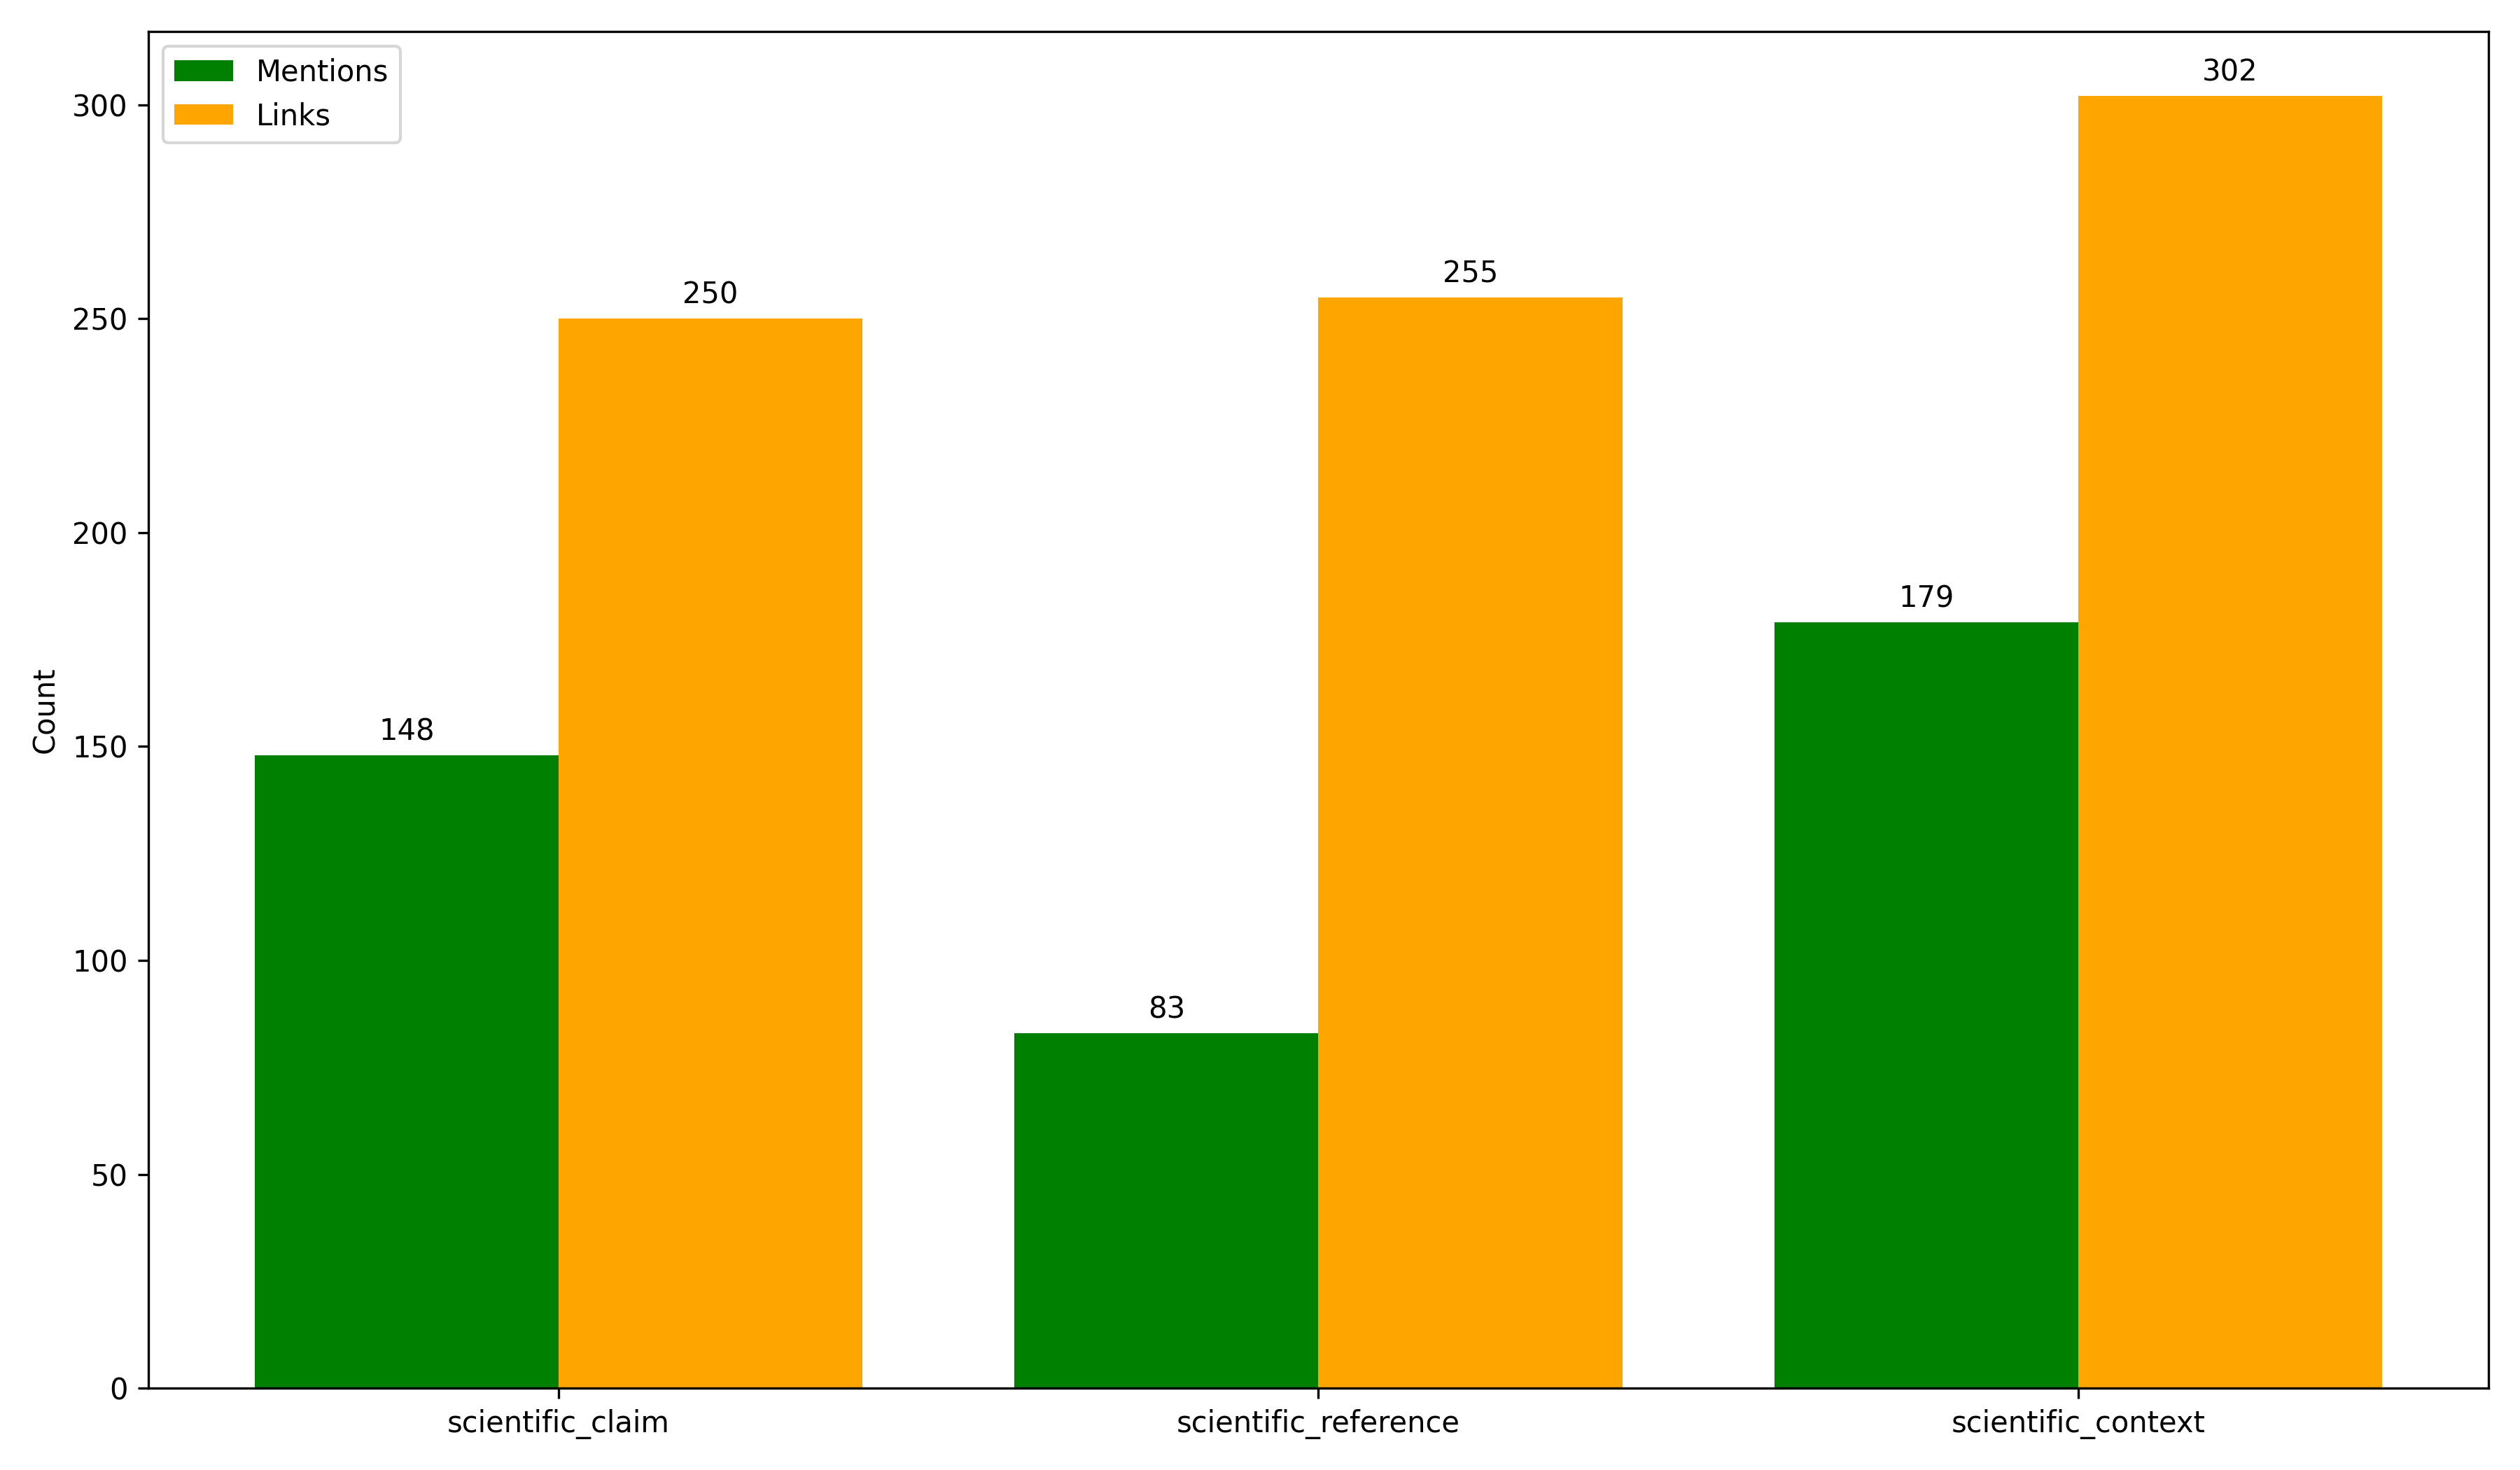
\includegraphics[width=1\textwidth]{images/hashtag_links_mentions_count_outliers}
    \caption{Nombre de hashtags par tweet selon le type de tweet scientifique.}
    \label{fig:hashtag_count}
\end{figure}

Après avoir réalisé des tests d'indépendance de student sur chaque variable, les \textit{p-values} ne descendent pas en dessous de 0.18 donc on ne remarque pas de différence significative entre les tweets scientifiques et non scientifiques.
On peut ainsi conclure que ces variables ne sont pas pertinentes pour la classification des tweets scientifiques, on les retirera de notre dataset.
Malgrès tout, les \texttt{\#} permettent une meilleur accuracy overall, on l'a donc gardé.

\subsection{Modélisation}\label{subsec:modelisation}
Dans cette section, nous comparons les performances des modèles sur trois tâches de classification hiérarchiques successives.
Par la suite, nous présentons les résultats de classification obtenus pour chaque tâche ainsi qu’une comparaison des performances des approches utilisées.

\noindent Pour chacunes des étapes, nous allons comparer différents modèles entre eux pour sélectionner le meilleur modèle.
Par meilleur modèle, on entend la meilleure précision et le plus petit écart-type.
Chaque modèle est testé par cross-validation sur 10 itérations.

\subsection{Tâche 1 : Classification binaire ({SCI} vs. {NON-SCI})}\label{subsec:modele-1:-sci-vs-non-sci}
Dans cette tâche, nous avons comparé plusieurs modèles de classification afin de distinguer les tweets scientifiques des non-scientifiques.
L’objectif était d’évaluer les performances de différentes approches d’apprentissage supervisé appliquées à un problème de classification binaire.

\subsubsection{Préparation des données}
Nous avons supprimé les mentions (@), les caractères spéciaux et converti l’ensemble des textes en minuscules, pour standardiser l’entrée pour éviter que des variations superficielles n’influencent la classification.
Une liste de stopwords a été utilisée, combinant celle de NLTK et des termes propres à Twitter ("http", "https", "rt", "co", "amp", "via") qui sont fréquents mais peu informatifs pour déterminer la nature scientifique du contenu.
Pour la vectorisation, nous avons utilisé la méthode TF-IDF avec des n-grammes de taille 1 à 2, un choix raisonnable pour capturer à la fois des mots individuels et des associations fréquentes, tout en limitant la complexité.

Étant donné le fort déséquilibre des classes (la classe SCI représentant moins de 10 \%), la technique SMOTE a été utilisée pour équilibrer la distribution entre classes SCI et NON-SCI.

\subsubsection{Analyse comparative des performances des différents modèles}
Plusieurs modèles de classification ont été testés (\autoref{tab:model_comparison_sci_nsci}).
Chacun a été optimisé à l’aide d’une recherche par grille (GridSearchCV) et évalué à l’aide d’une validation croisée à 10 plis (KFold), afin d’identifier les meilleures combinaisons d’hyperparamètres.

\begin{table}[H]
    \centering
    \caption{Performances des modèles - Tâche 1 (KFold = 10)}
    \begin{tabular}{lcccc}
        \toprule
        Modèle & Accuracy (\autoref{fig:model_comparison_sci_nsci}) & Précision (\autoref{fig:confusion_1.json-SVM_sci_confusion_matrix}) & Rappel (\autoref{fig:confusion_1.json-SVM_sci_confusion_matrix}) & F1-score \\
        \midrule
        Logistic Regression & 0.9327 ± 0.0163 & 0.93 & 0.93 & 0.93 \\
        Naive Bayes & 0.9118 ± 0.0197 & 0.91 & 0.90 & 0.89 \\
        k-NN & 0.8111 ± 0.0286 & 0.82 & 0.79 & 0.78 \\
        Random Forest & 0.8575 ± 0.0246 & 0.89 & 0.86 & 0.86 \\
        SVM & \textbf{0.9431 ± 0.0137} & \textbf{0.92} & \textbf{0.92} & \textbf{0.92} \\
        \bottomrule
    \end{tabular}\label{tab:model_comparison_sci_nsci}
\end{table}

\noindent Le modèle SVM semble être le plus performant pour cette tâche, affichant les meilleurs scores en précision, rappel et F1-score, ainsi qu’une accuracy élevée accompagnée du plus faible écart-type.
Ces performances stables, observées à la fois sur le jeu de test et au cours de la validation croisée, sont clairement visibles dans le boxplot (\autoref{fig:model_comparison_sci_nsci}).
En comparaison, la régression logistique s’est également montrée très efficace, représentant une alternative pertinente, notamment dans des cas où l’on recherche un bon compromis entre précision et rappel.

\vfill
\begin{figure}[H]
    \centering
    \begin{minipage}[b]{0.55\textwidth}
        \centering
        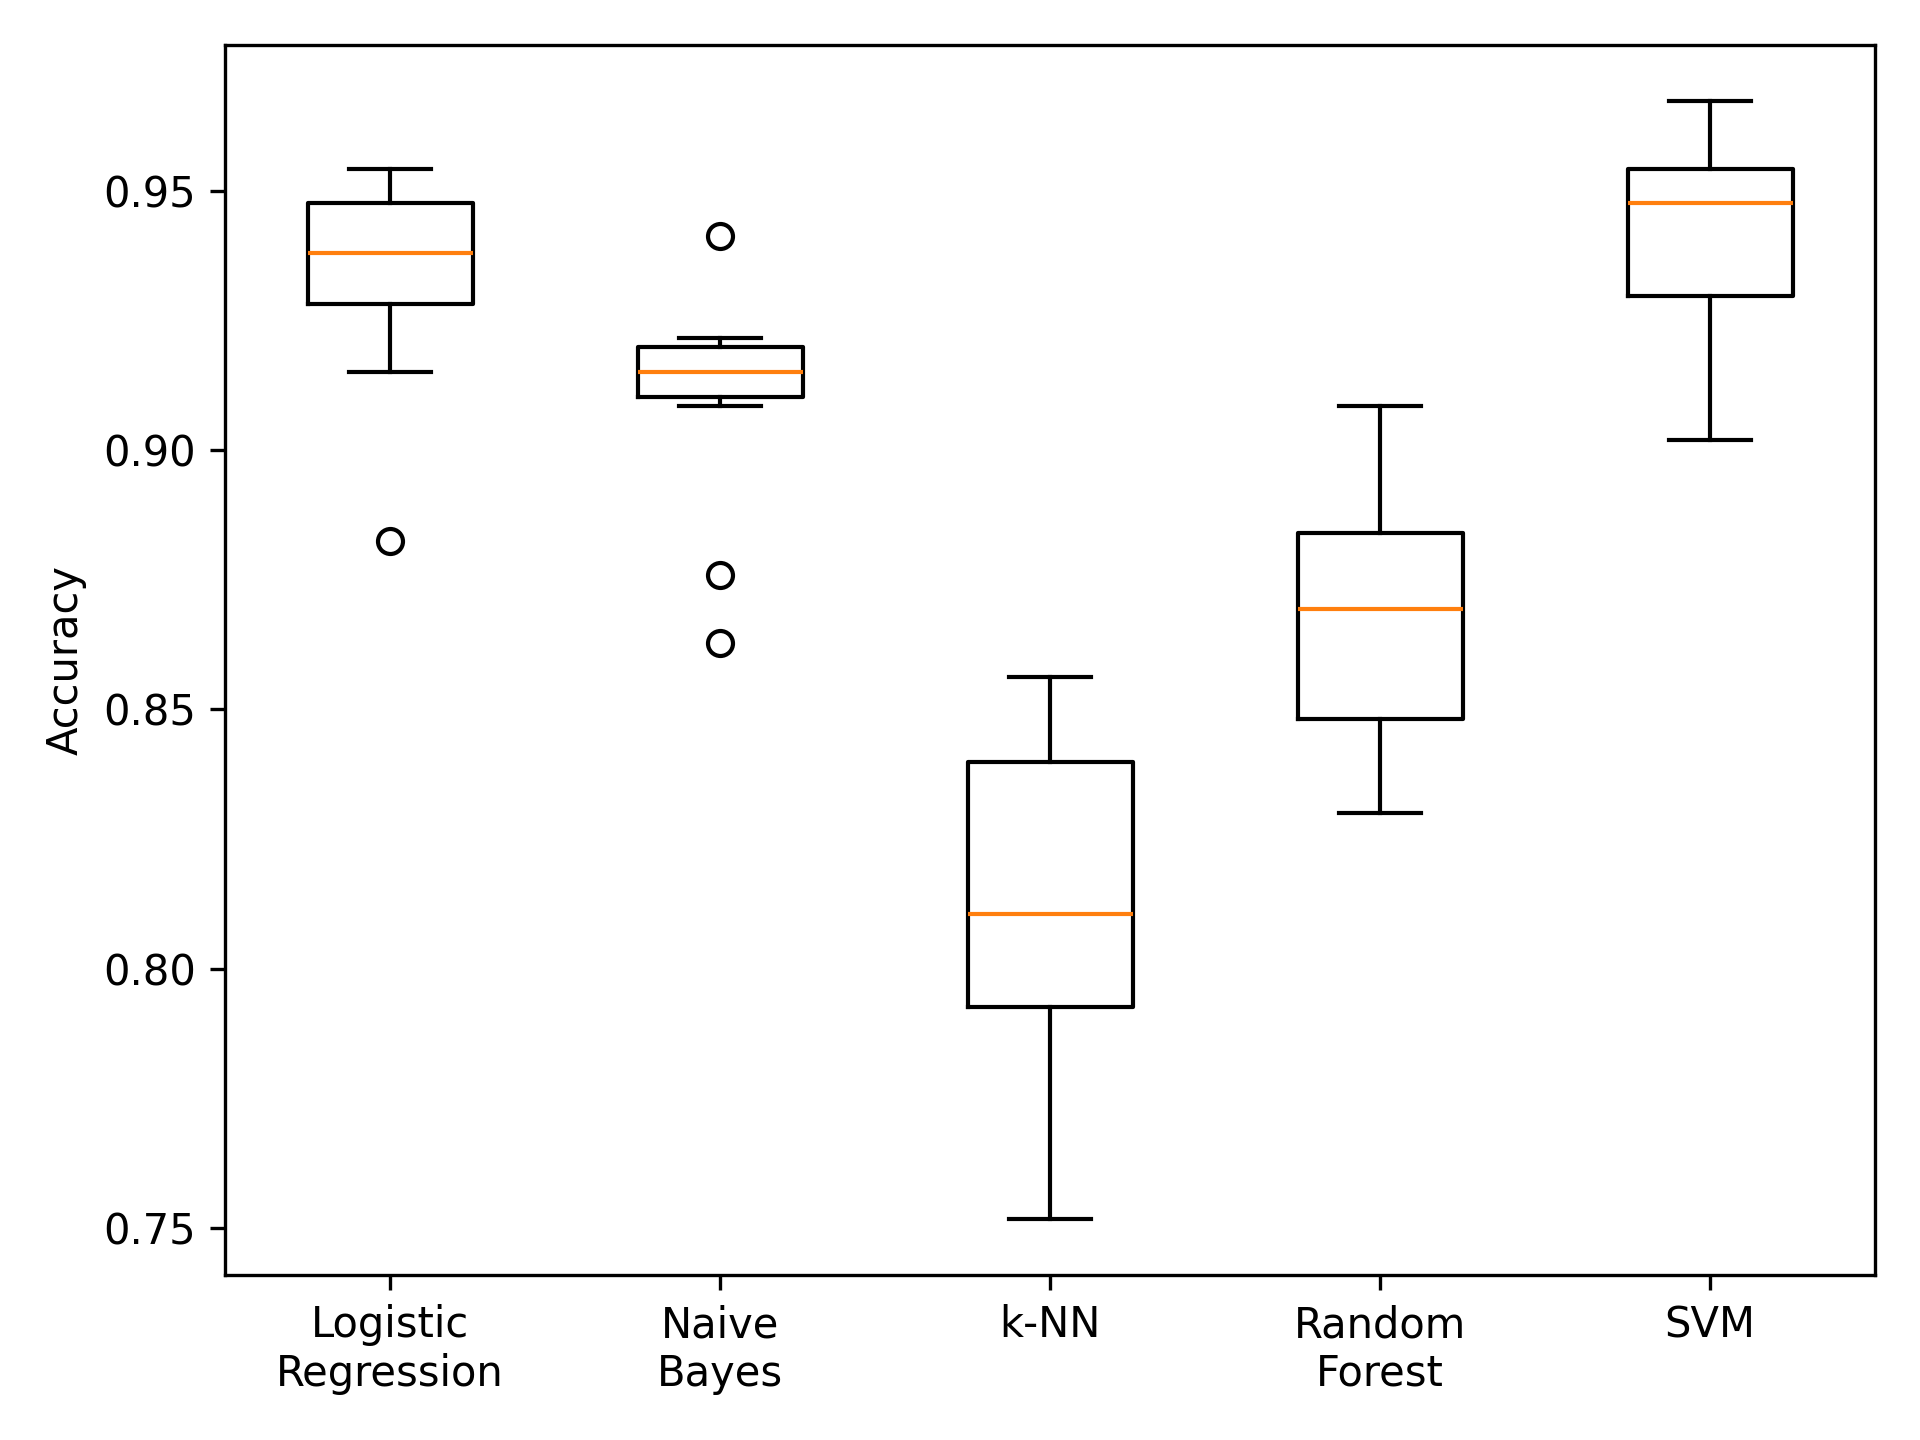
\includegraphics[width=\textwidth]{images/model_comparison_1}
        \caption{Comparaison des modèles pour la classification des tweets scientifiques et non scientifiques.}
        \label{fig:model_comparison_sci_nsci}
    \end{minipage}\hfill
    \begin{minipage}[b]{0.4\textwidth}
        \centering
        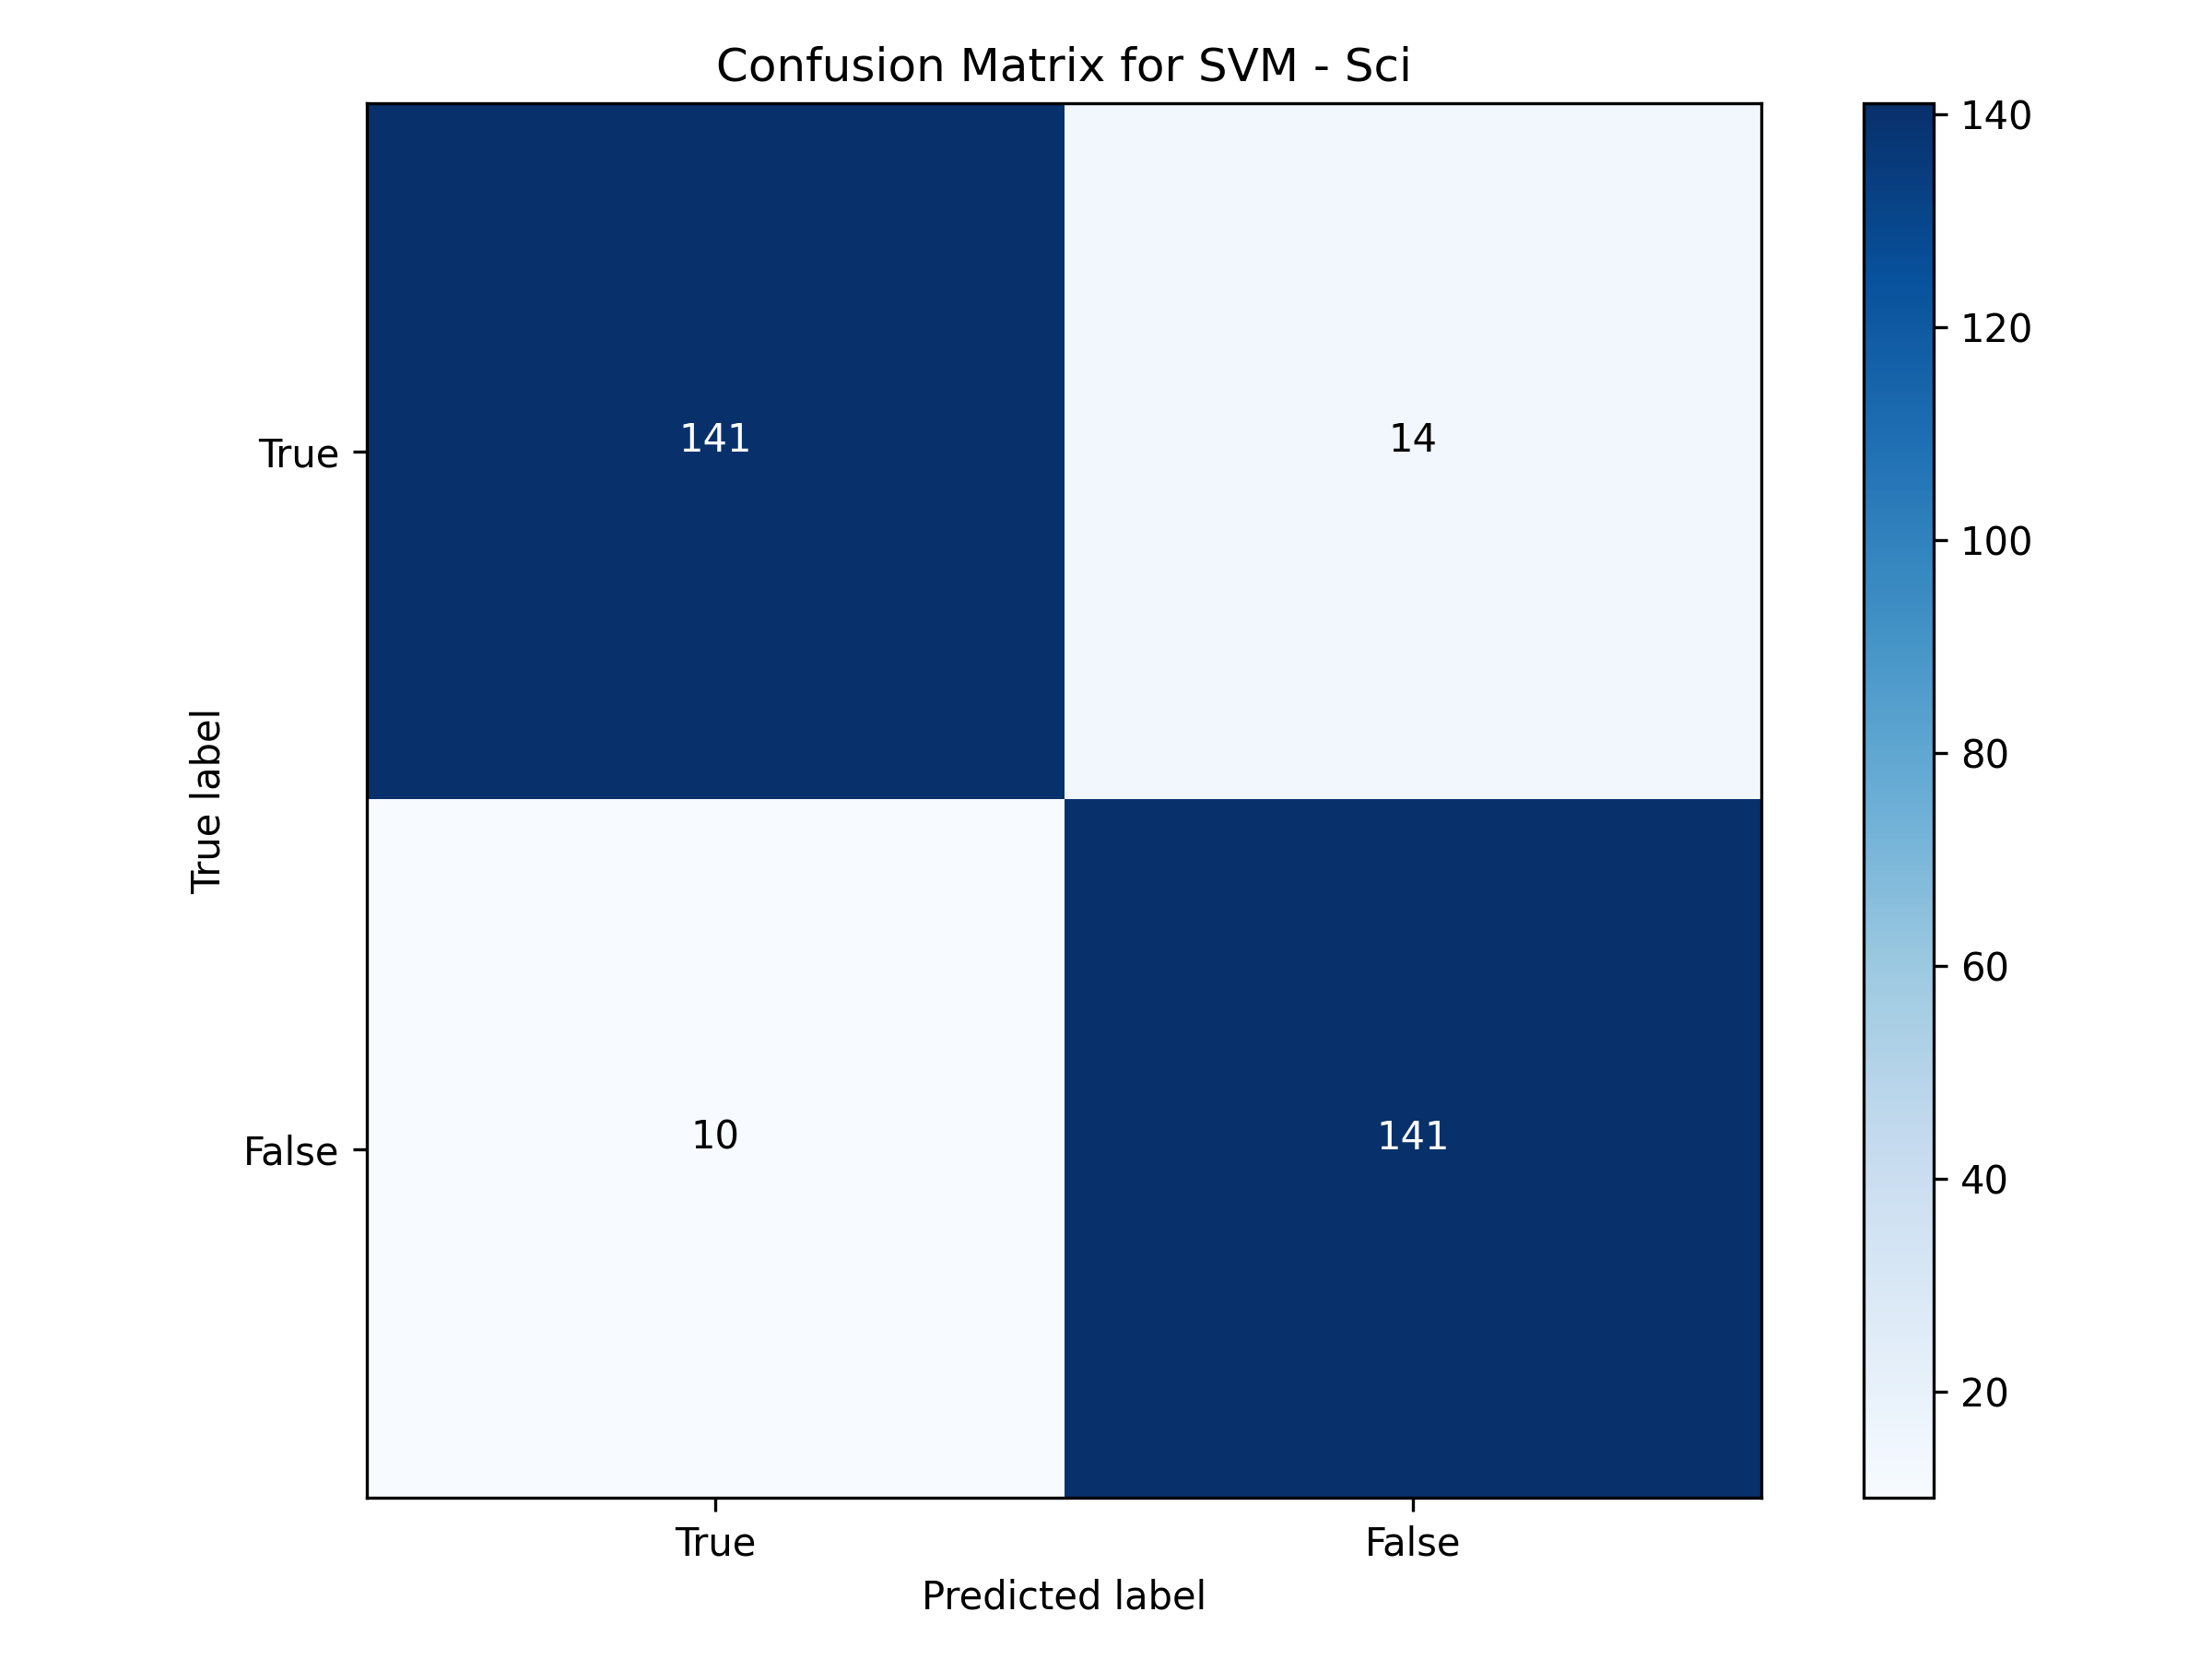
\includegraphics[width=\textwidth]{images/confusion_1.json-SVM_Sci_confusion_matrix}
        \caption{Matrice de confusion du modèle SVM pour la classification des tweets scientifiques et non scientifiques.}
        \label{fig:confusion_1.json-SVM_sci_confusion_matrix}
    \end{minipage}
\end{figure}
\newpage

\subsection{Tâche 2 : Classification Binaire Multi-Label ({CLAIM, REF} vs. {CONTEXT})}\label{subsec:modele-2:-claim-et-ref-vs-contexte}
À présent, nous allons considérer les classes "Affirmation" et "Référence" qui citent une affirmation scientifique d’une part, et la classe "Contexte" qui servent de contexte
D’autre part, toujours afin de réaliser une classification binaire.
Les tweets analysés sont uniquement ceux classés comme scientifiques dans la première tâche.

\subsubsection{Préparation des données}
Le prétraitement textuel a suivi une logique proche de celle adoptée dans la première tâche (minuscules, stop words, lemmatisation), mais sans suppression des mentions et caractères spéciaux, afin d’explorer s’ils peuvent porter une valeur contextuelle utile.
La vectorisation a été réalisée à l’aide de TF-IDF, en élargissant la fenêtre aux trigrammes (1 à 3-grammes) pour mieux capturer les structures linguistiques propres aux énoncés de type affirmation ou citation.

Contrairement à la première tâche, nous n’avons pas appliqué SMOTE ici, le déséquilibre est partiel dans la distribution des combinaisons de labels.
La classification est multi-label (un tweet peut être à la fois CONTEXT et CLAIM/REF).
Nous avons donc implémenté un rééchantillonnage manuel spécifique au multi-label, en nous basant sur l’identification de toutes les combinaisons de labels possibles et en suréchantillonnant celles qui étaient sous-représentées.

\subsubsection{Analyse comparative des performances des différents modèles}
Dans cette deuxième tâche, nous avons comparé plusieurs modèles de classification pour résoudre un problème de classification multi-label, où chaque tweet peut être associé à plusieurs catégories (\autoref{tab:model_comparison_clmref_context})
L’objectif était d’évaluer l’efficacité de différentes approches d’apprentissage supervisé adaptées à ce type de problème.

\begin{table}[H]
    \centering
    \caption{Performances - Tâche 2}
    \begin{tabular}{lcccc}
        \toprule
        Modèle & Accuracy & Précision & Rappel & F1-score \\
        \midrule
        SVM & 0.9183 ± 0.0193 & 0.99 & 1.00 & 0.99 \\
        Naive Bayes & 0.8647 ± 0.0292 & 0.93 & 0.93 & 0.93 \\
        k-NN & 0.8876 ± 0.0183 & 0.99 & 0.99 & 0.99 \\
        Random Forest & 0.9359 ± 0.0162 & 0.99 & 1.00 & 0.99 \\
        Logistic Regression & 0.8961 ± 0.0232 & 0.98 & 0.97 & 0.97 \\
        Gradient Boosting & \textbf{0.9236 ± 0.0162} & \textbf{0.99} & \textbf{1.00} & \textbf{0.99} \\
        \bottomrule
    \end{tabular}\label{tab:model_comparison_clmref_context}
\end{table}

Le modèle Gradient Boosting a montré des performances supérieures dans le cadre de ce problème de classification binaire, atteignant une précision globale de 0.97 et un rappel parfait de 1.00 pour la classe 'claim\_or\_ref'.
L'optimisation des hyperparamètres à l'aide de GridSearchCV a permis d'affiner les paramètres clés, tels que le learning rate (0.1) et la profondeur maximale (5), pour obtenir un score de validation croisée de 0.9236, garantissant une excellente généralisation.
En comparaison avec d'autres modèles comme le SVM et le Random Forest, qui ont également montré des performances solides, le Gradient Boosting s'est distingué par sa capacité à mieux gérer les classes déséquilibrées et à produire des résultats plus équilibrés.
Bien que le k-NN ait présenté des résultats impressionnants avec des scores de précision et de rappel élevés (0.99), il a montré un léger sur-apprentissage, ce qui peut poser un problème avec de très grands ensembles de données.

\begin{figure}[H]
    \centering
    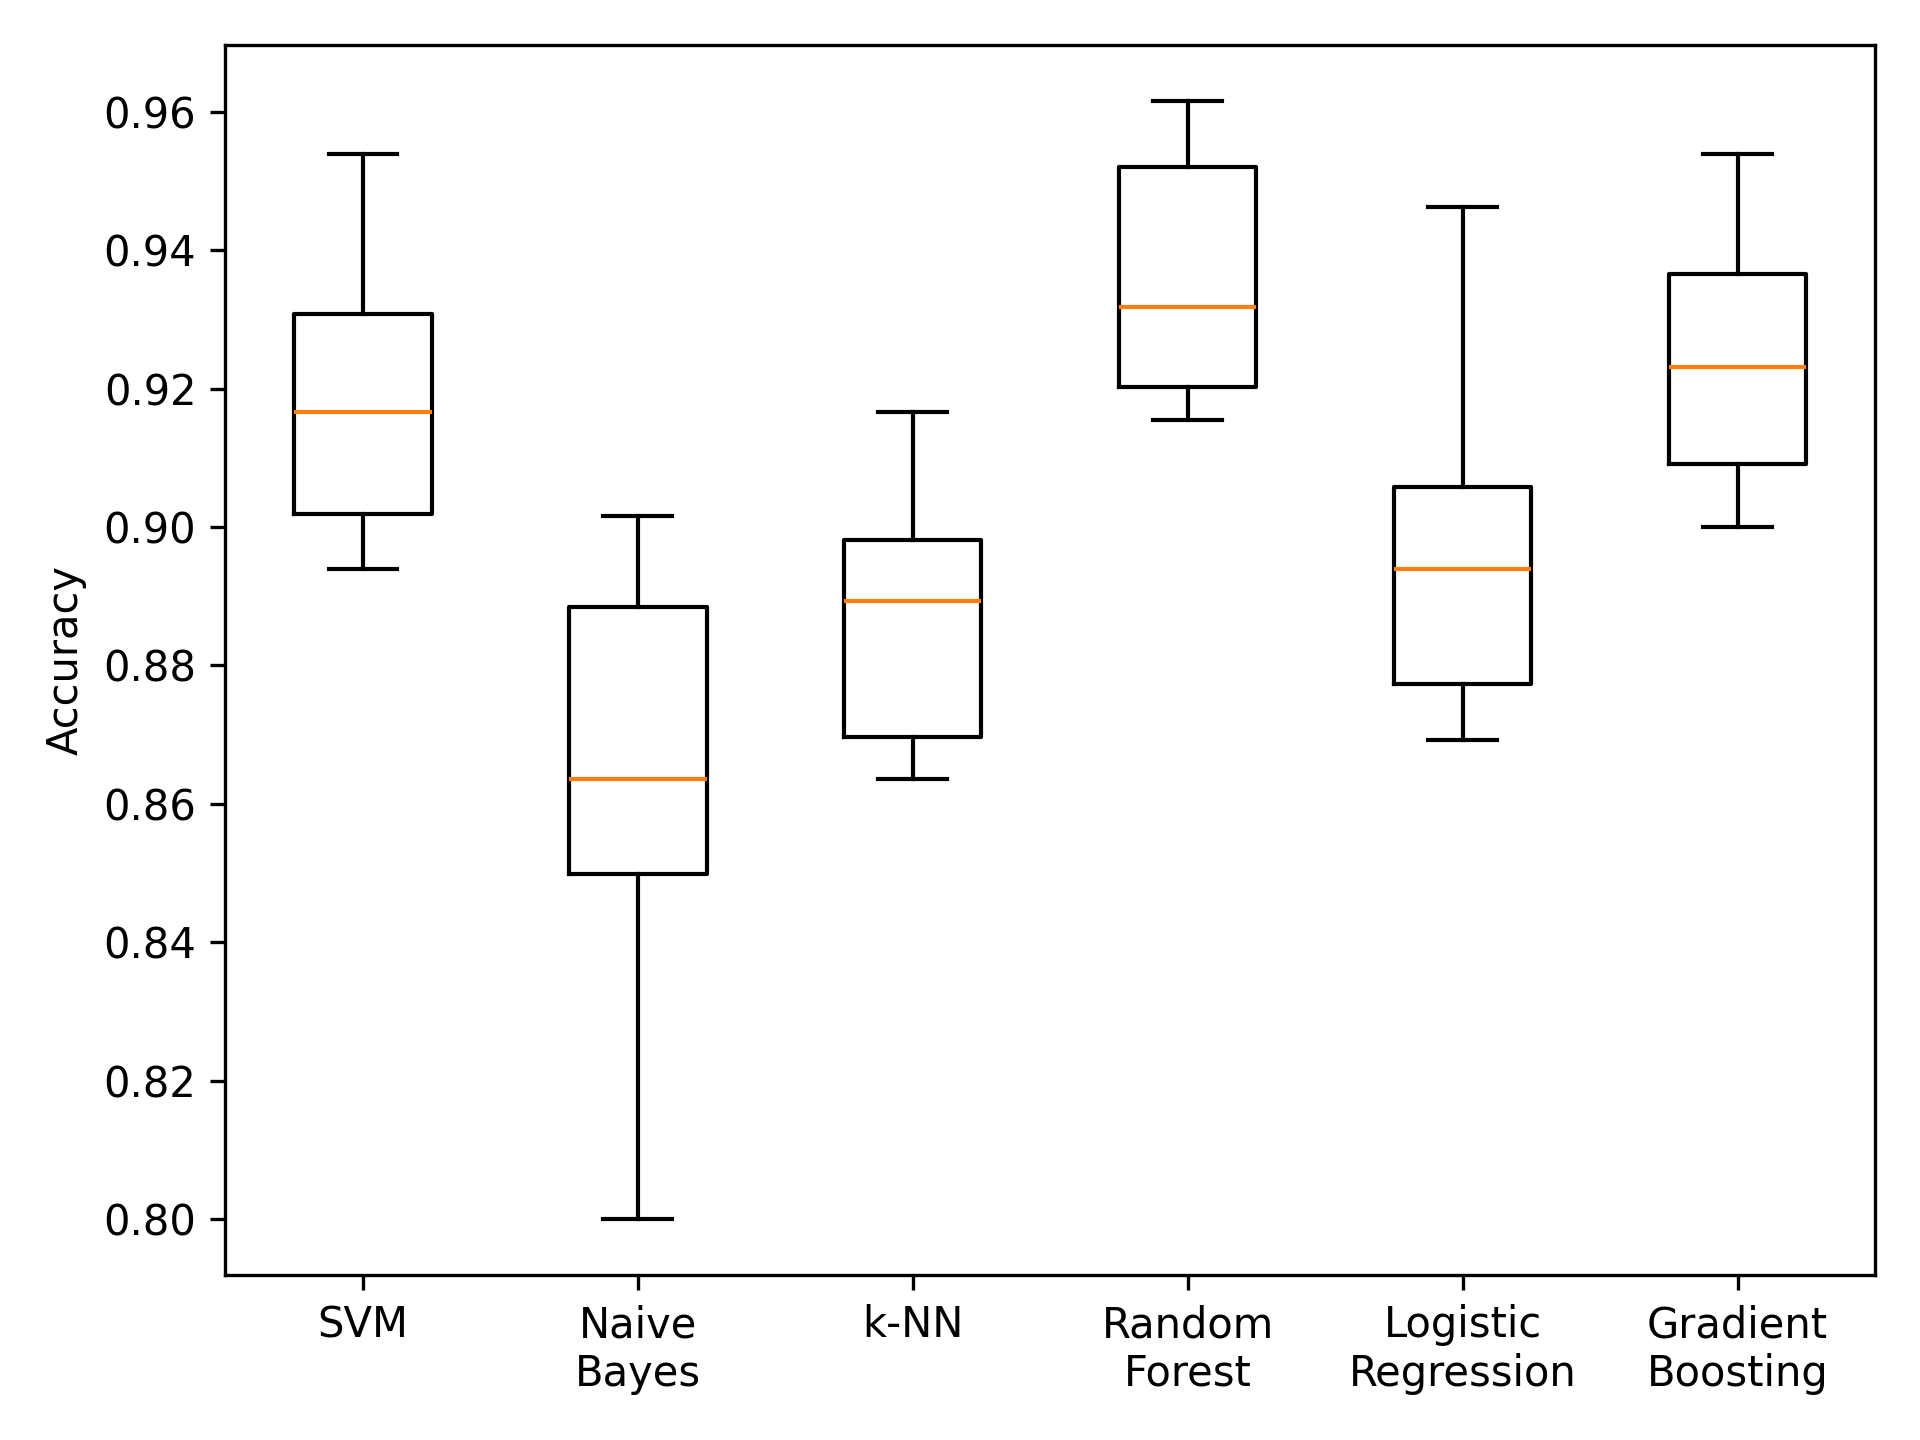
\includegraphics[width=0.75\textwidth]{images/model_comparison_2}
    \caption{Comparaison des modèles pour la classification des tweets claim et ref vs contexte.}
    \label{fig:model_comparison_clmref_context}
\end{figure}

\begin{figure}[h]
    \centering
    \begin{minipage}[b]{0.49\textwidth}
        \centering
        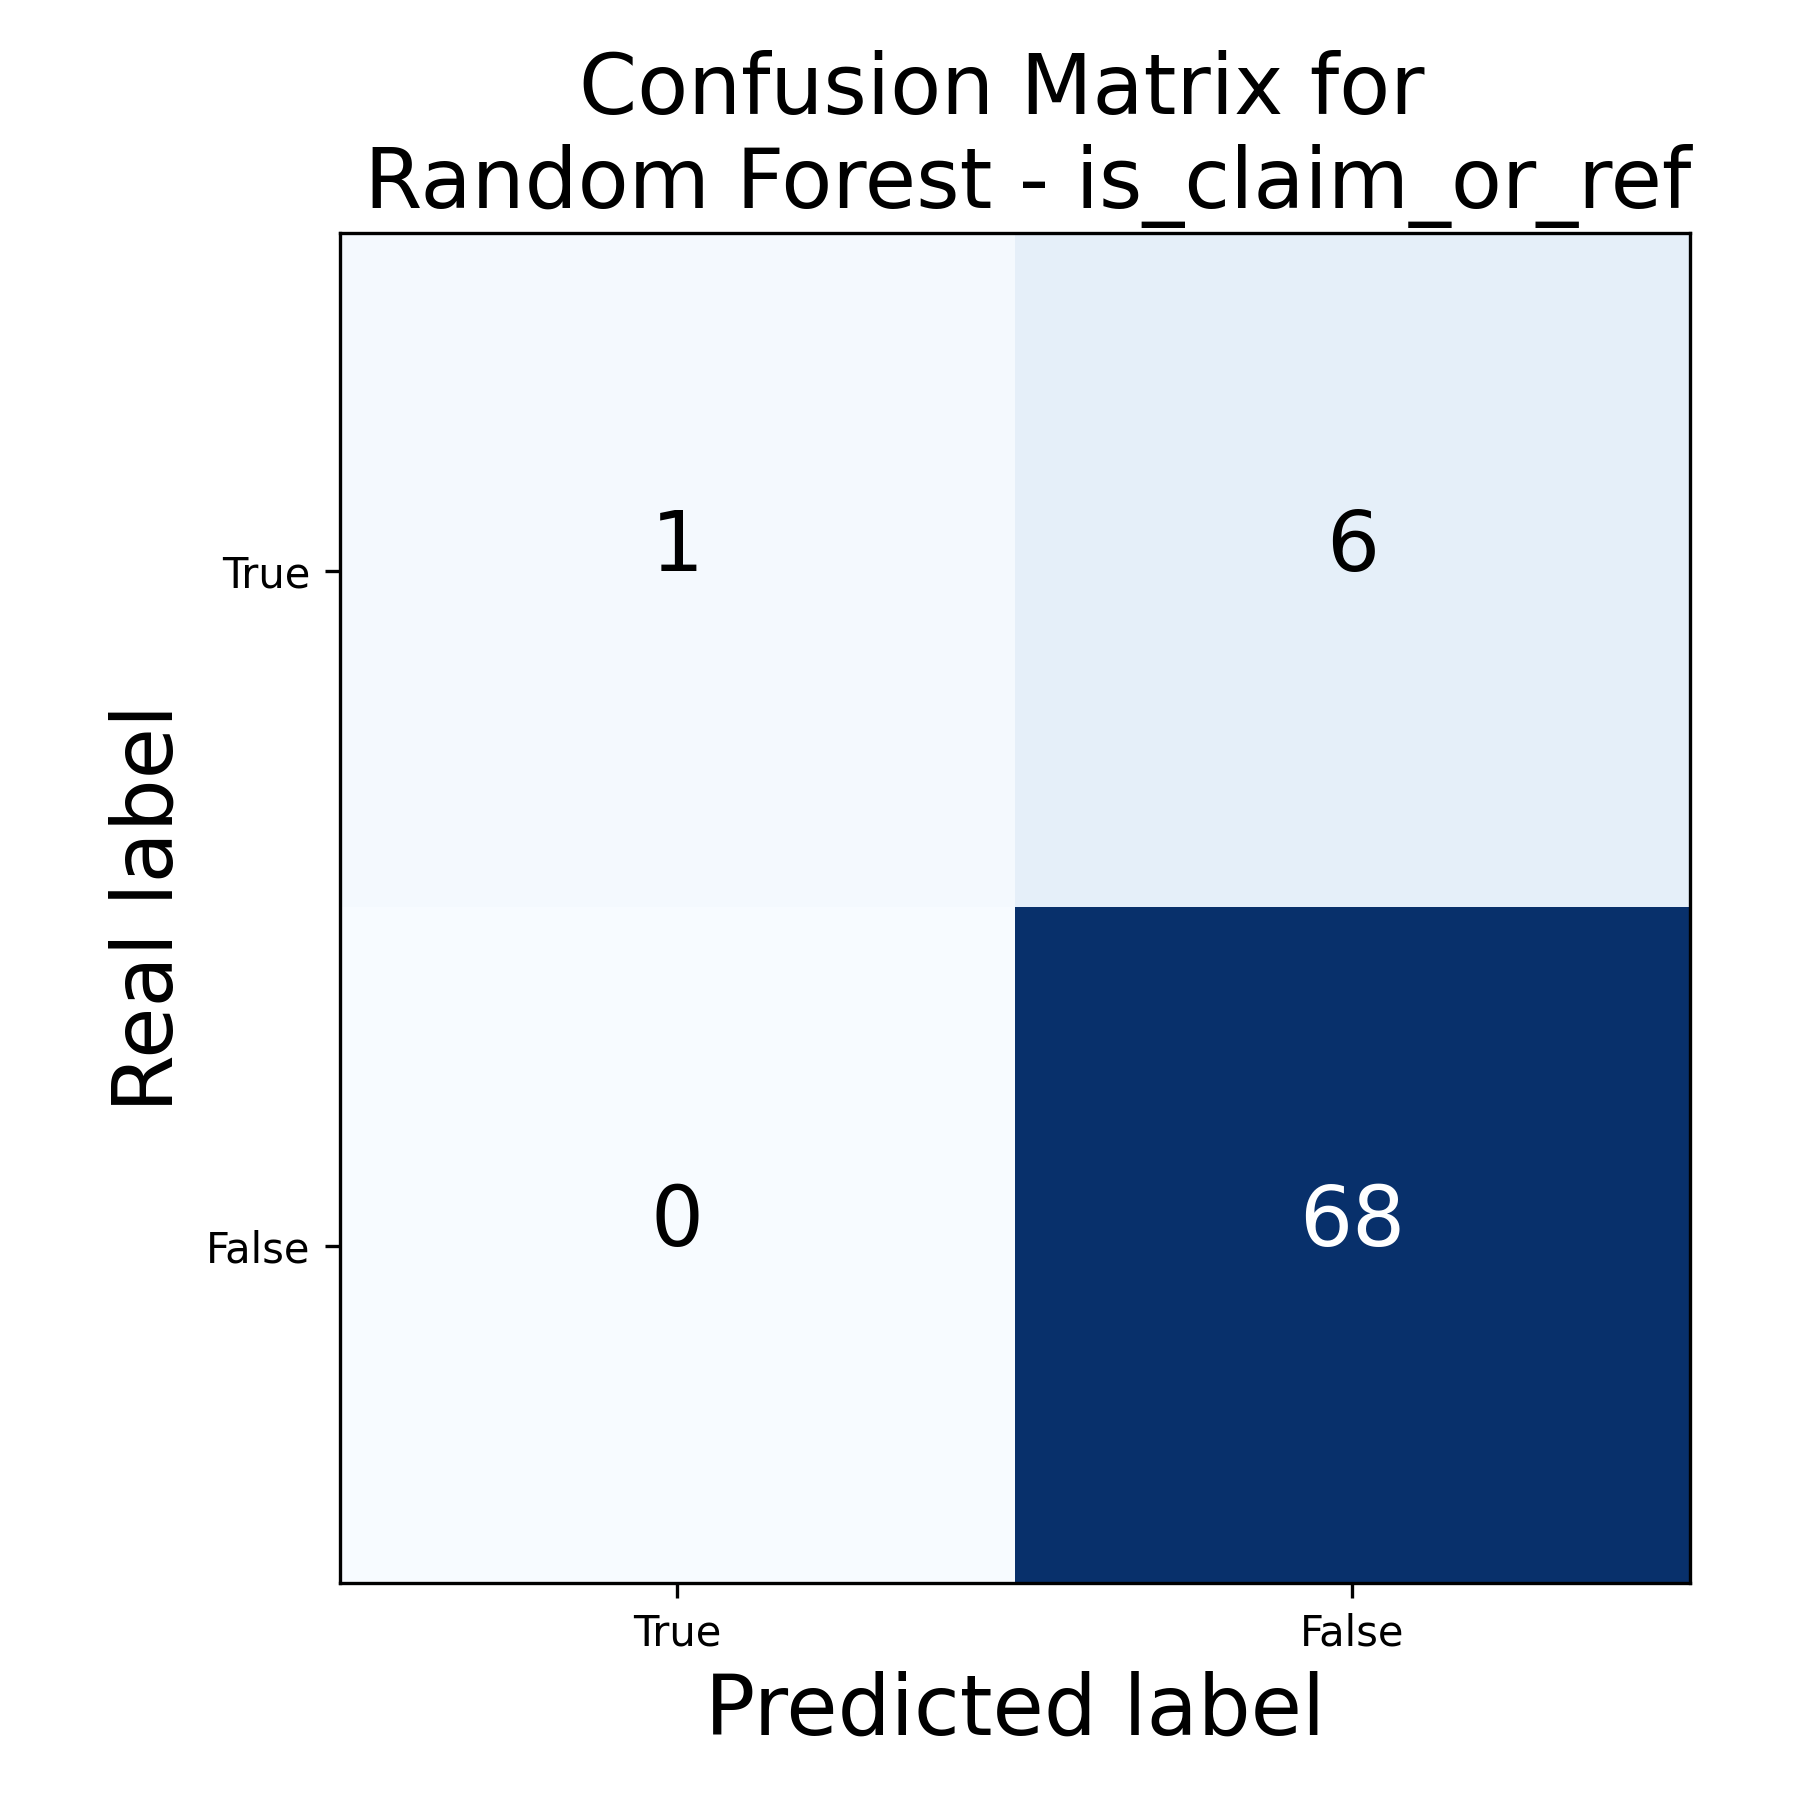
\includegraphics[width=\textwidth]{images/confusion_2.json-Random Forest_is_claim_or_ref_confusion_matrix}
        \label{fig:confusion_2_1}
    \end{minipage}
    \hfill
    \begin{minipage}[b]{0.49\textwidth}
        \centering
        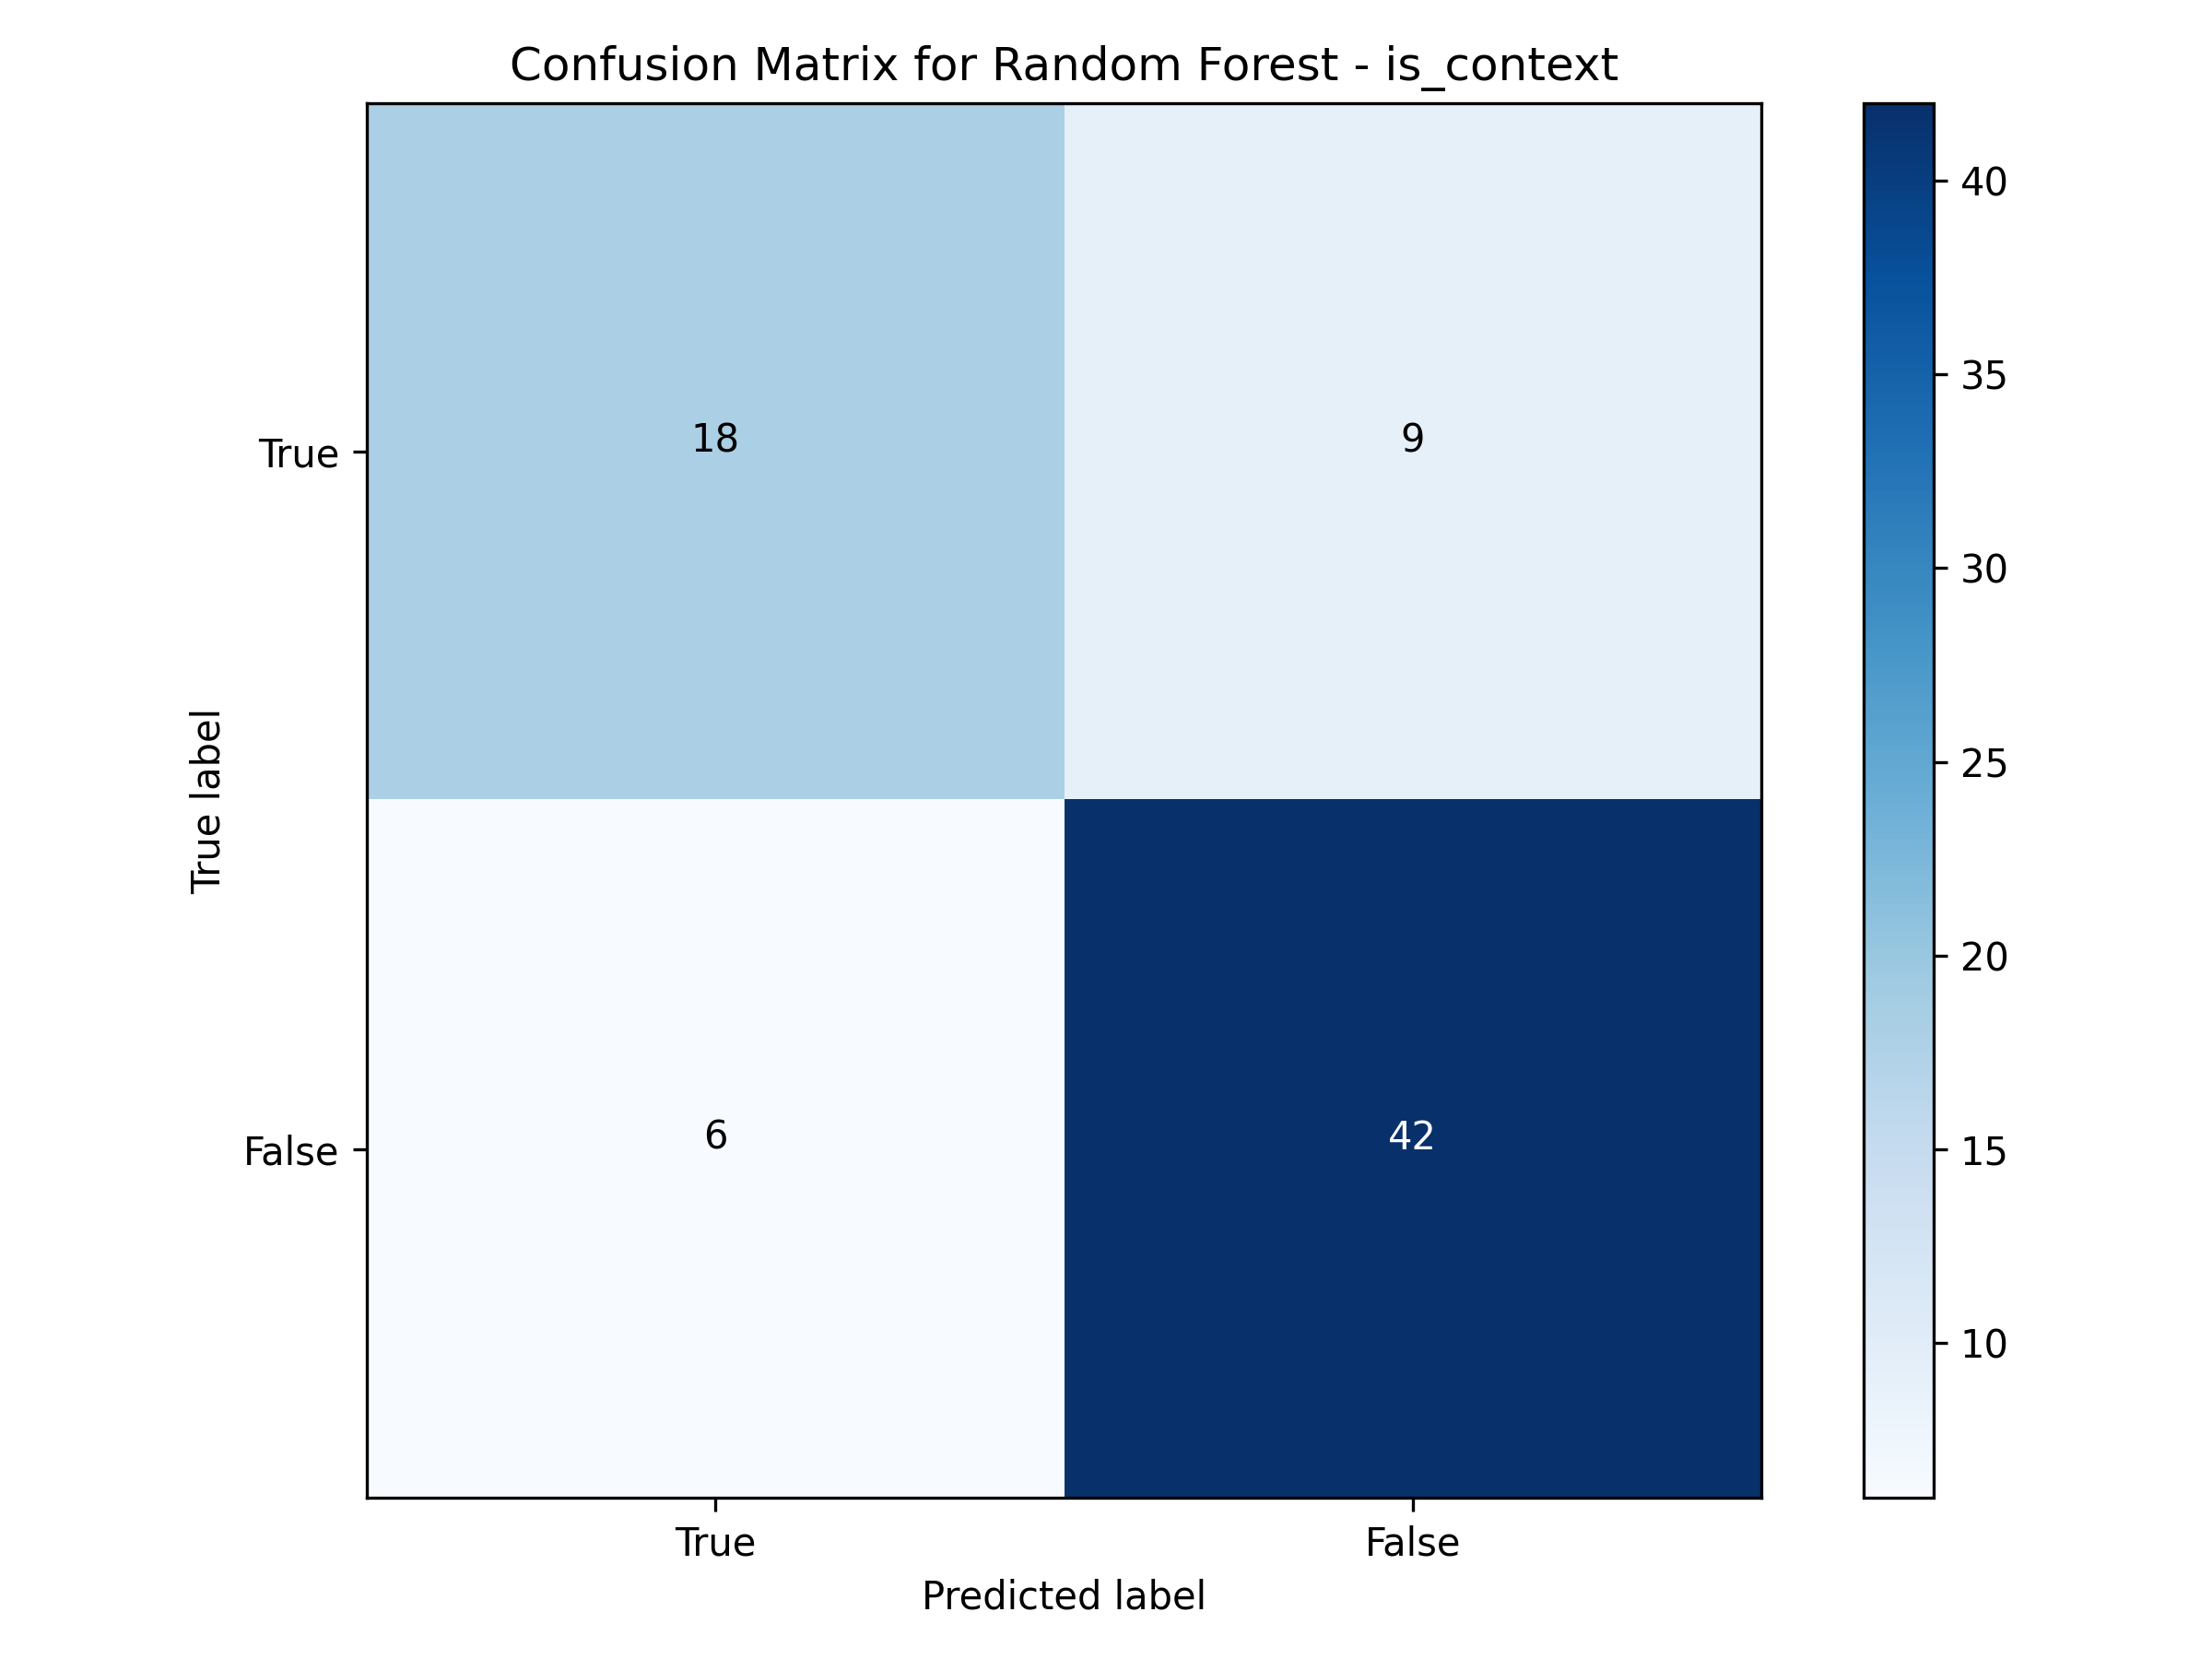
\includegraphics[width=\textwidth]{images/confusion_2.json-Random Forest_is_context_confusion_matrix}
        \label{fig:confusion_2_2}
    \end{minipage}
    \caption{Matrice de confusion du modèle Random Forest pour la classification des tweets claim et ref vs contexte.}
    \label{fig:confusion_2}
\end{figure}

\subsection{Tâche 3 :classification multi-classe et multi-label non exclusive ({CLAIM} vs. {REF} vs. {CONTEXT})}\label{subsec:modele-3:-claim-vs-ref-vs-contexte}
Cette dernière tâche est la plus fine du projet : elle consiste à classer chaque tweet scientifique selon trois catégories : Affirmation, Référence ou Contexte.
Bien qu’il s’agisse d’une classification à trois classes, le problème reste de nature multi-label, car un même tweet peut appartenir à plusieurs catégories simultanément.

\subsubsection{Préparation des données}
Le prétraitement a suivi une démarche classique, avec une étape supplémentaire pour la classe REF, qui était moins bien prédite.

\noindent À cette fin, les URLs ont été remplacées par le token "URL", afin d’en conserver la trace (utile pour reconnaître les références) sans inclure les chaînes brutes.
Les stop words ont été nettoyés à l’aide d’une liste enrichie (incluant des termes fréquents sur Twitter comme "rt", "co", "amp", "via", tout en veillant à conserver les négations, susceptibles de porter des nuances importantes.
La vectorisation s’est appuyée sur un TF-IDF intégrant des n-grammes allant jusqu’à trois mots, les trigrammes étant particulièrement efficaces pour différencier entre REF (souvent formalisé), CLAIM (langage 	assertif) et CONTEXT (vocabulaire plus descriptif).
Enfin, en raison du déséquilibre marqué entre les catégories (par exemple, très peu de REF), on a implémenté un suréchantillonnage manuel par combinaison de labels, sans détruire la nature multi-étiquette.

\subsubsection{Analyse comparative des performances des différents modèles}
\begin{table}[H]
    \centering
    \caption{Performances - Tâche 3}
    \begin{tabular}{lcccc}
        \toprule
        Modèle & Accuracy & Hamming Loss & F1-score & Rappel \\
        \midrule
        LinearSVC & 0.7171 ± 0.0625 & 0.2844 ± 0.0625 & 0.8844 ± 0.0625 & 0.75 ± 0.04 \\
        Random Forest & \textbf{0.7836 ± 0.0507} & 0.2489 ± 0.0507 & \textbf{0.9133 ± 0.0507} & 0.83 ± 0.05 \\
        SVM & 0.7331 ± 0.0691 & 0.2622 ± 0.0691 & 0.8992 ± 0.0691 & \textbf{0.89 ± 0.07} \\
        Naive Bayes & 0.6101 ± 0.0802 & 0.3156 ± 0.0802 & 0.8601 ± 0.0802 & 0.82 ± 0.07 \\
        k-NN & 0.6868 ± 0.0763 & 0.36 ± 0.0763 & 0.8615 ± 0.0763 & 0.77 ± 0.06 \\
        Logistic Regression & 0.7433 ± 0.0545 & 0.2578 ± 0.0545 & 0.8933 ± 0.0545 & 0.79 ± 0.06 \\
        Gradient Boosting & 0.7696 ± 0.0476 & \textbf{0.2356 ± 0.0476} & 0.9086 ± 0.0476 & 0.85 ± 0.05 \\
        \bottomrule
    \end{tabular}\label{tab:model_comparison_clm_ref_context}
\end{table}

Dans cette tâche, tous les modèles de classification présentent une précision et un F1-score relativement bons.
On remarque en revanche des valeurs de Hamming Loss plus faibles pour des modèles comme Random Forest, Gradient Boosting et Logistic Regression.
Ceci indique une capacité à mieux classer les données tout en minimisant les erreurs globales.

\noindent La précision est généralement élevée pour les classes claim et context, mais elle est un peu plus faible pour la classe reference, ce qui peut expliquer pourquoi ces modèles ont des performances variées.
Cela montre que les modèles sont bons pour identifier les assertions et les contextes, mais ont plus de difficulté à classer correctement les références.
Ceci peut être dû à une classe reference plus difficile à différencier ou moins représentée dans le jeu de données.

Cependant, le F1-score est parfois un peu plus élevé que le score d'accuracy.
Les modèles cherchent à optimiser un compromis entre précision et rappel pour chaque classe.

La Hamming Loss plus élevée pour des modèles comme k-NN et Naive Bayes est probablement le reflet de leur difficulté à bien distinguer toutes les classes.
Particulièrement pour la classe reference, qui semble poser plus de défis en termes de précision et de rappel.
Cela explique aussi pourquoi ces modèles, bien que performants dans certaines classes, peuvent avoir des scores globaux de précision et de rappel moins élevés par rapport à d'autres.
En effet, Random Forest ou Gradient Boosting, paraissent mieux gérer la classification dans l’ensemble.

\begin{figure}[H]
    \centering
    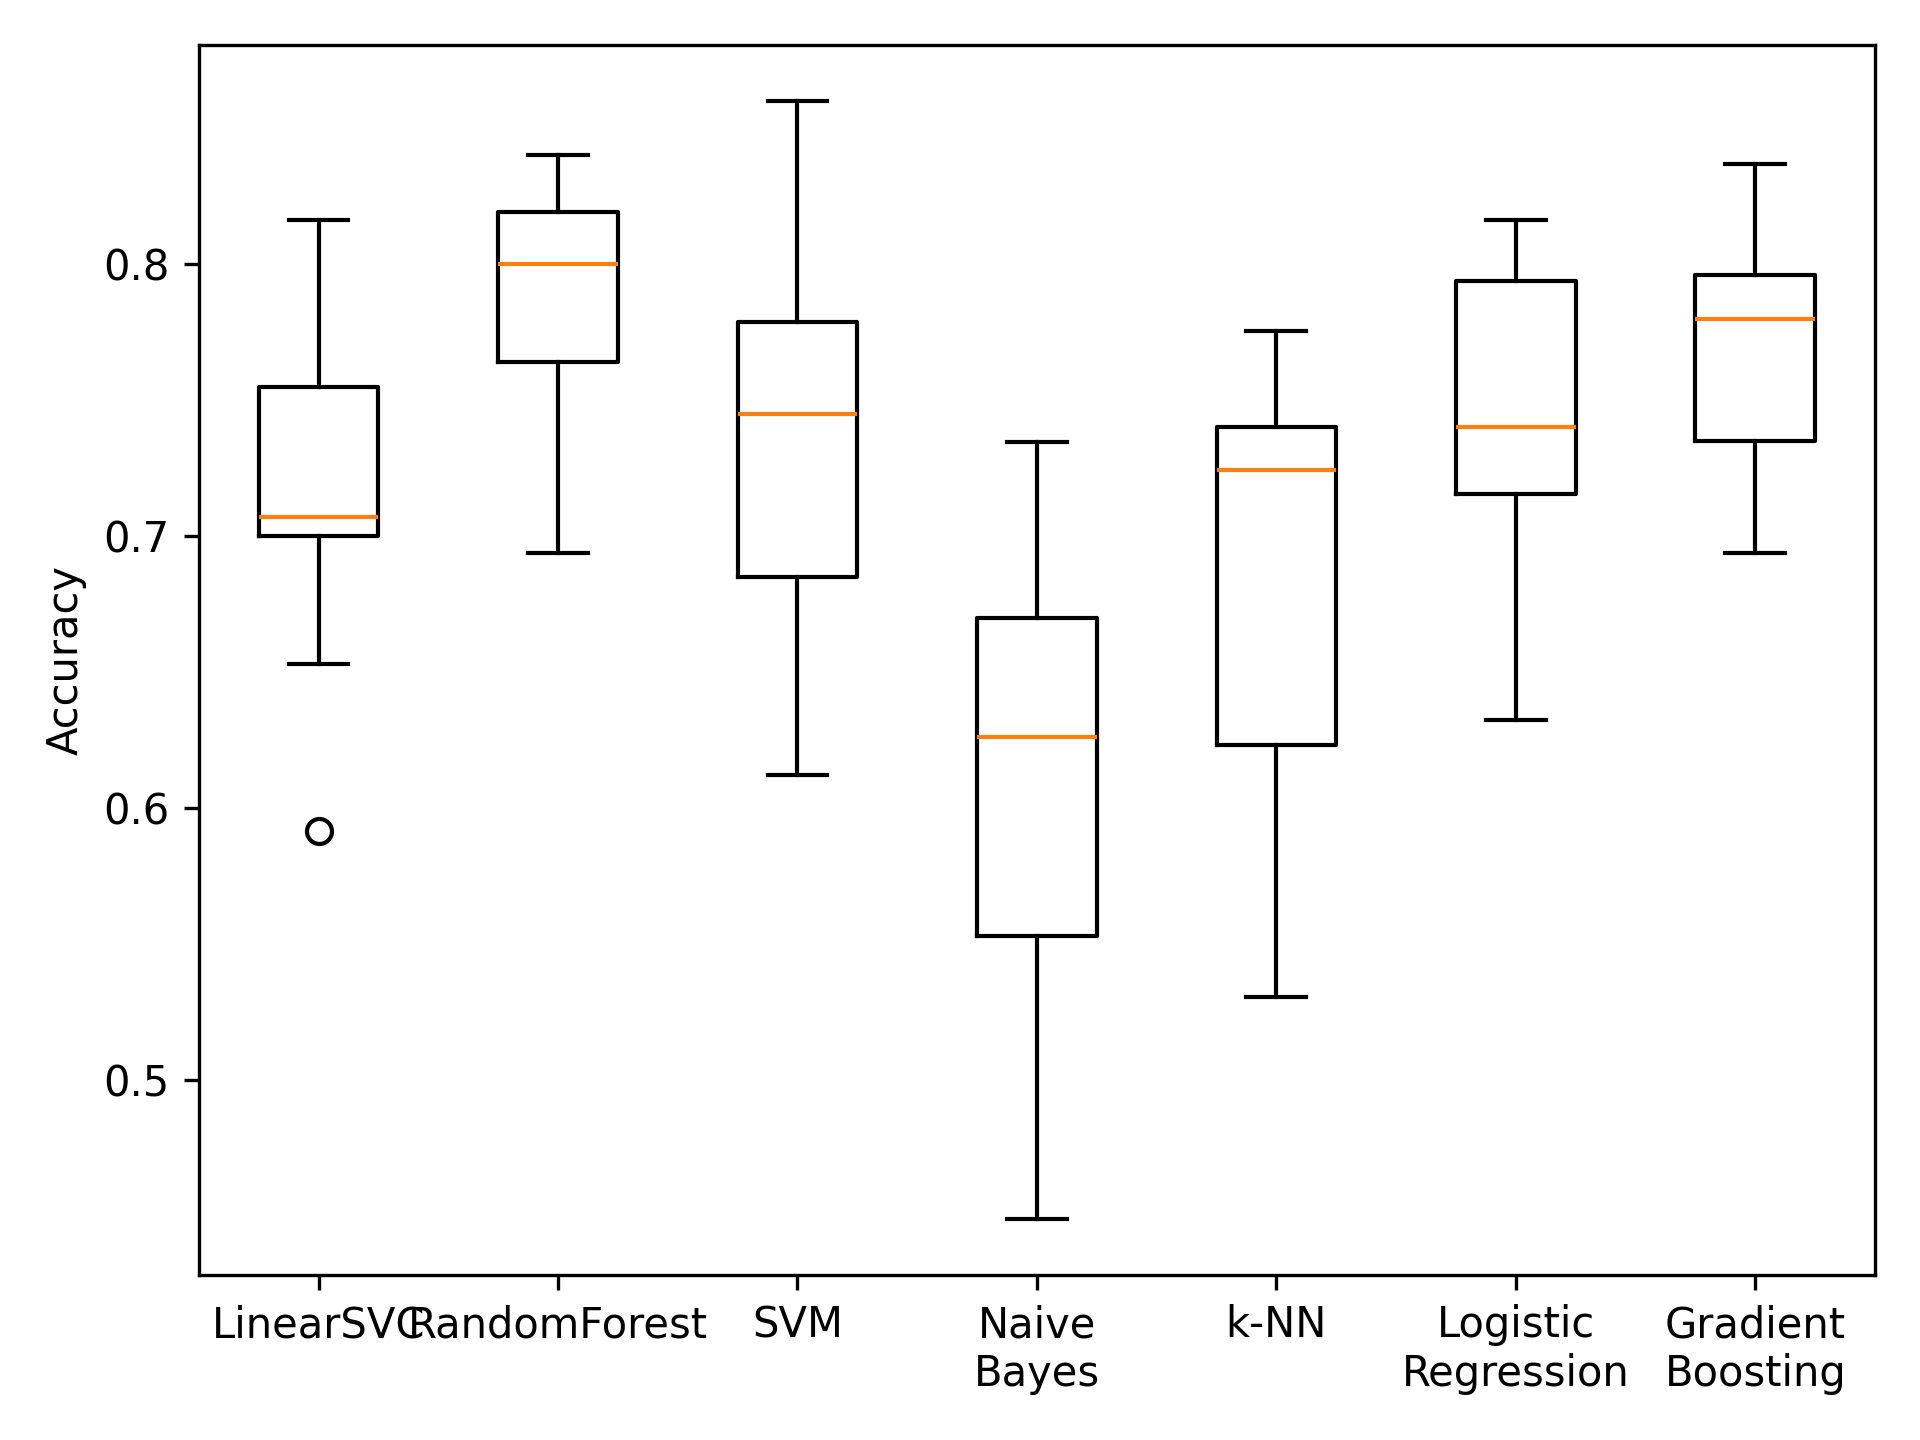
\includegraphics[width=0.75\textwidth]{images/model_comparison_3}
    \caption{Comparaison des modèles pour la classification des tweets claim vs ref vs contexte.}
    \label{fig:model_comparison_clm_ref_context}
\end{figure}

\begin{figure}[h]
    \centering
    \begin{minipage}[b]{0.3\textwidth}
        \centering
        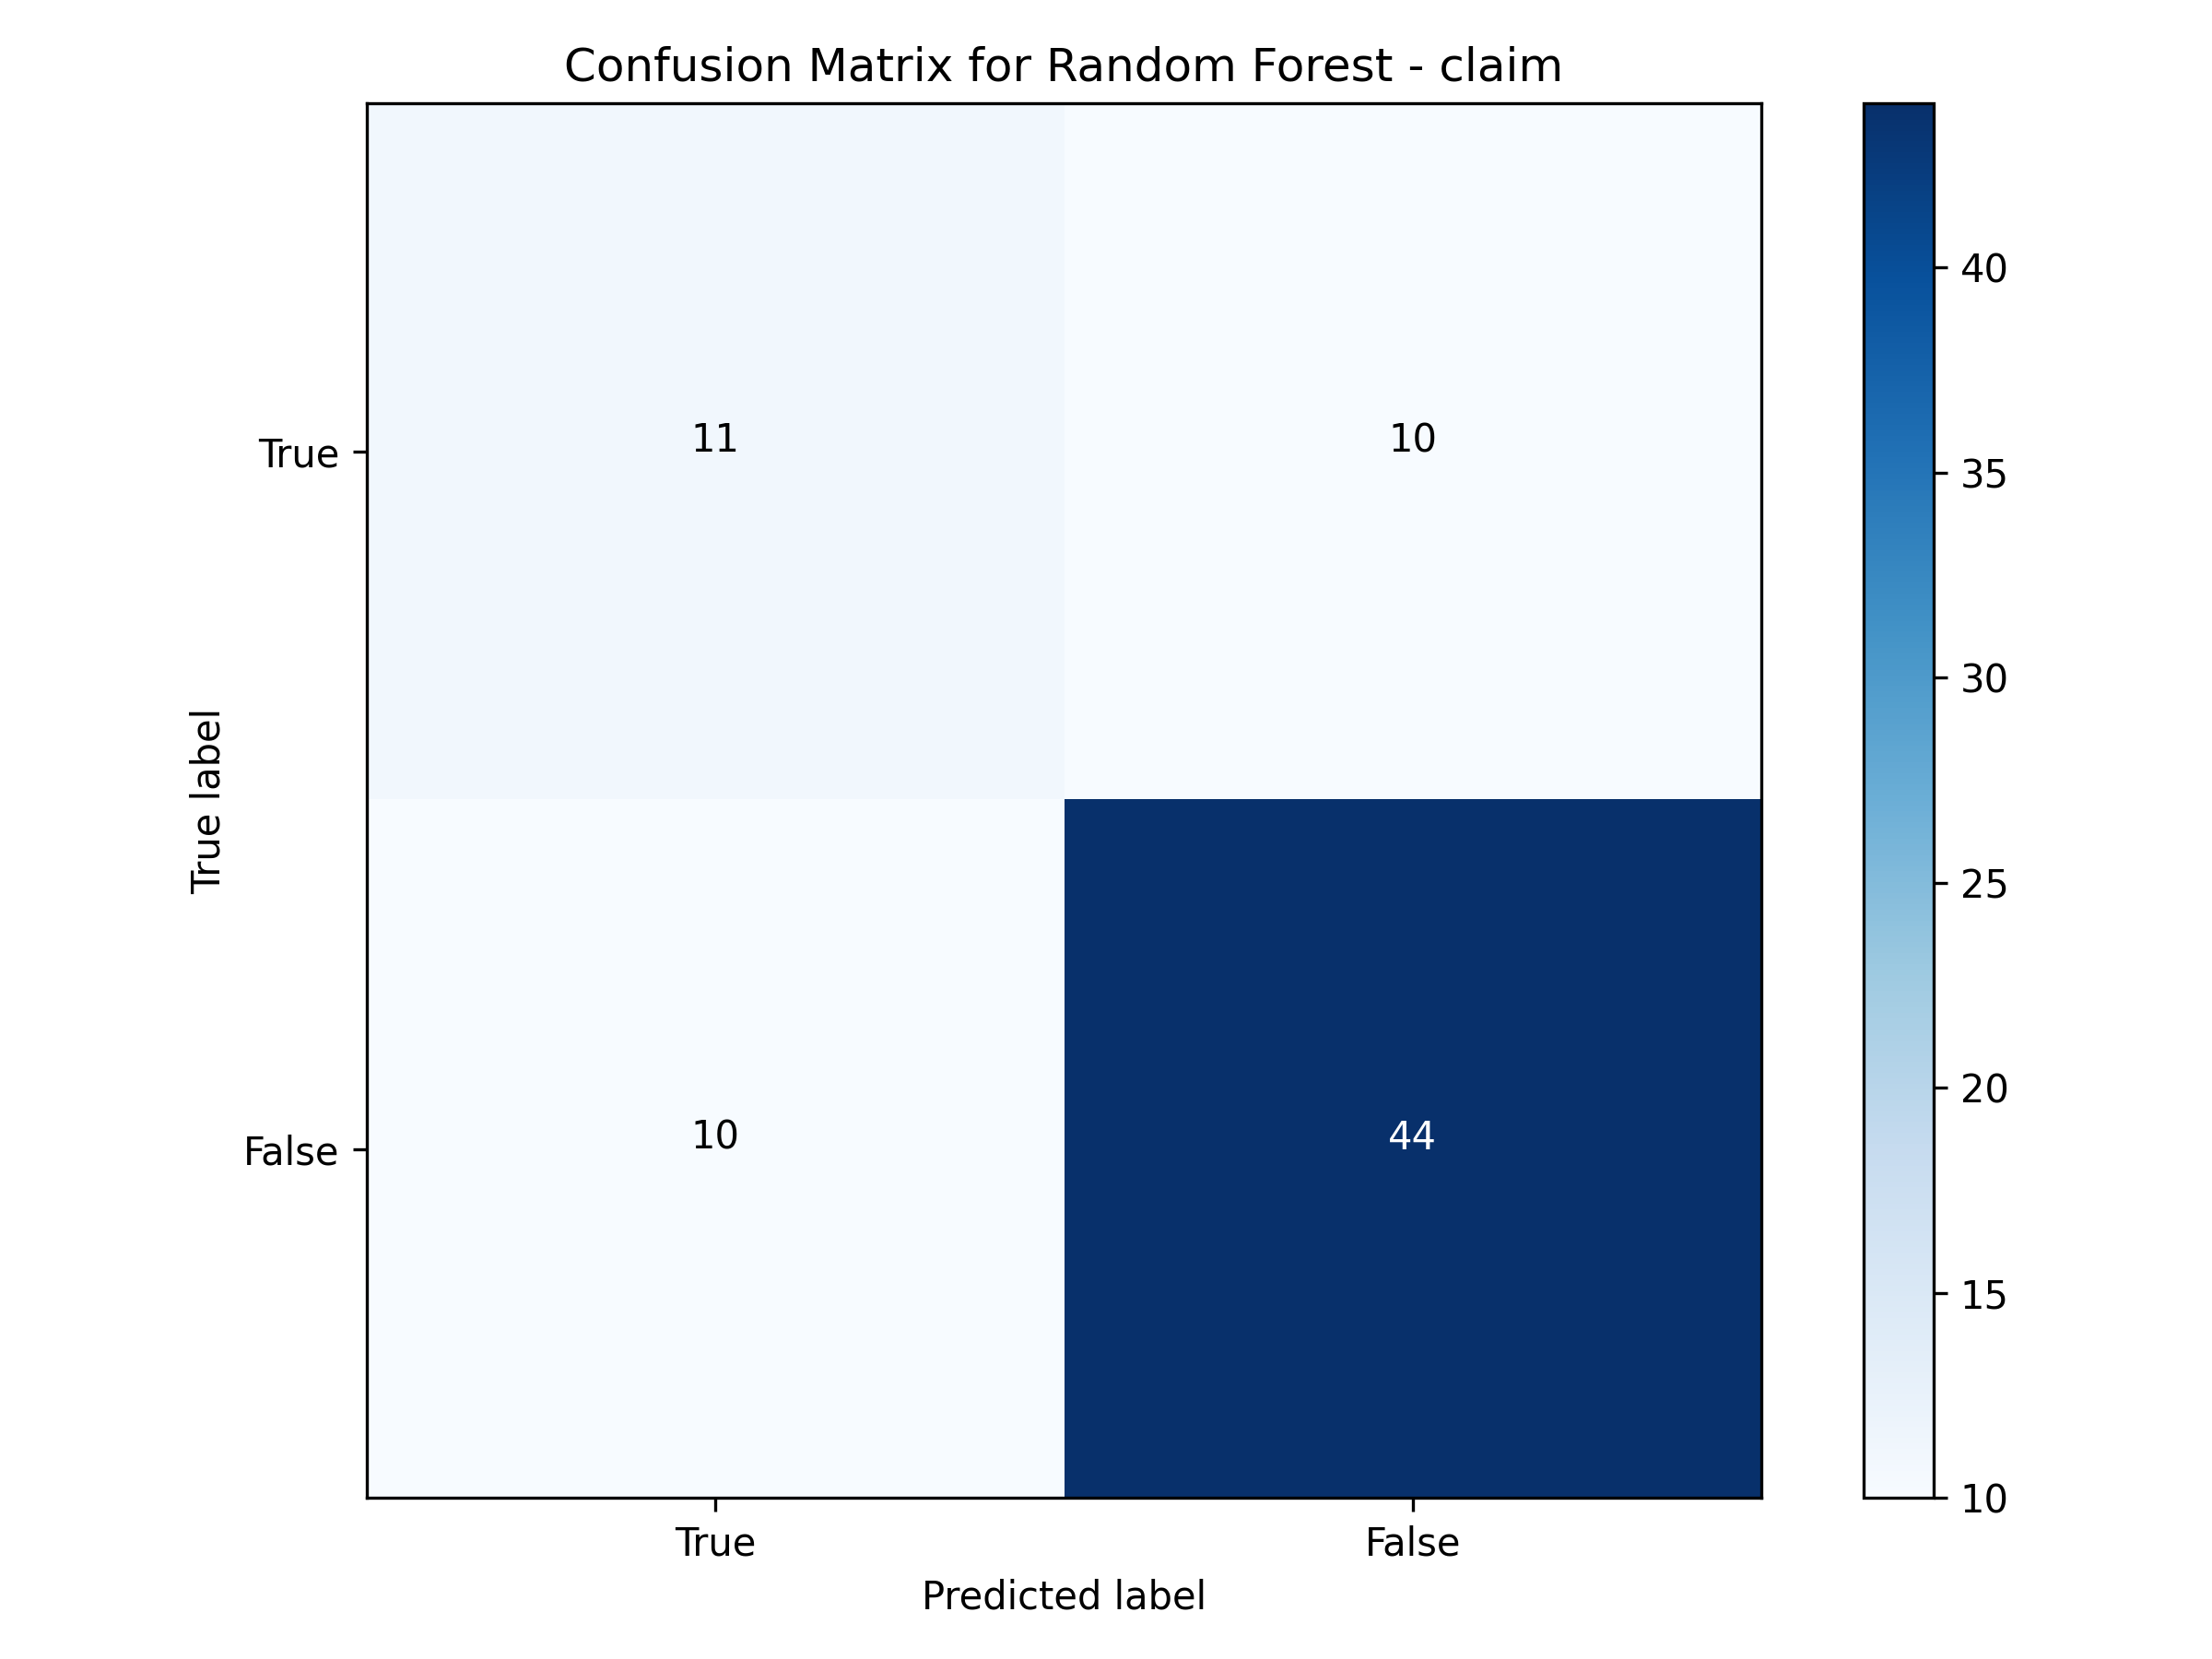
\includegraphics[width=\textwidth]{images/confusion_3.json-Random Forest_claim_confusion_matrix}
        \label{fig:confusion_3_1}
    \end{minipage}
    \hspace{1em}
    \begin{minipage}[b]{0.3\textwidth}
        \centering
        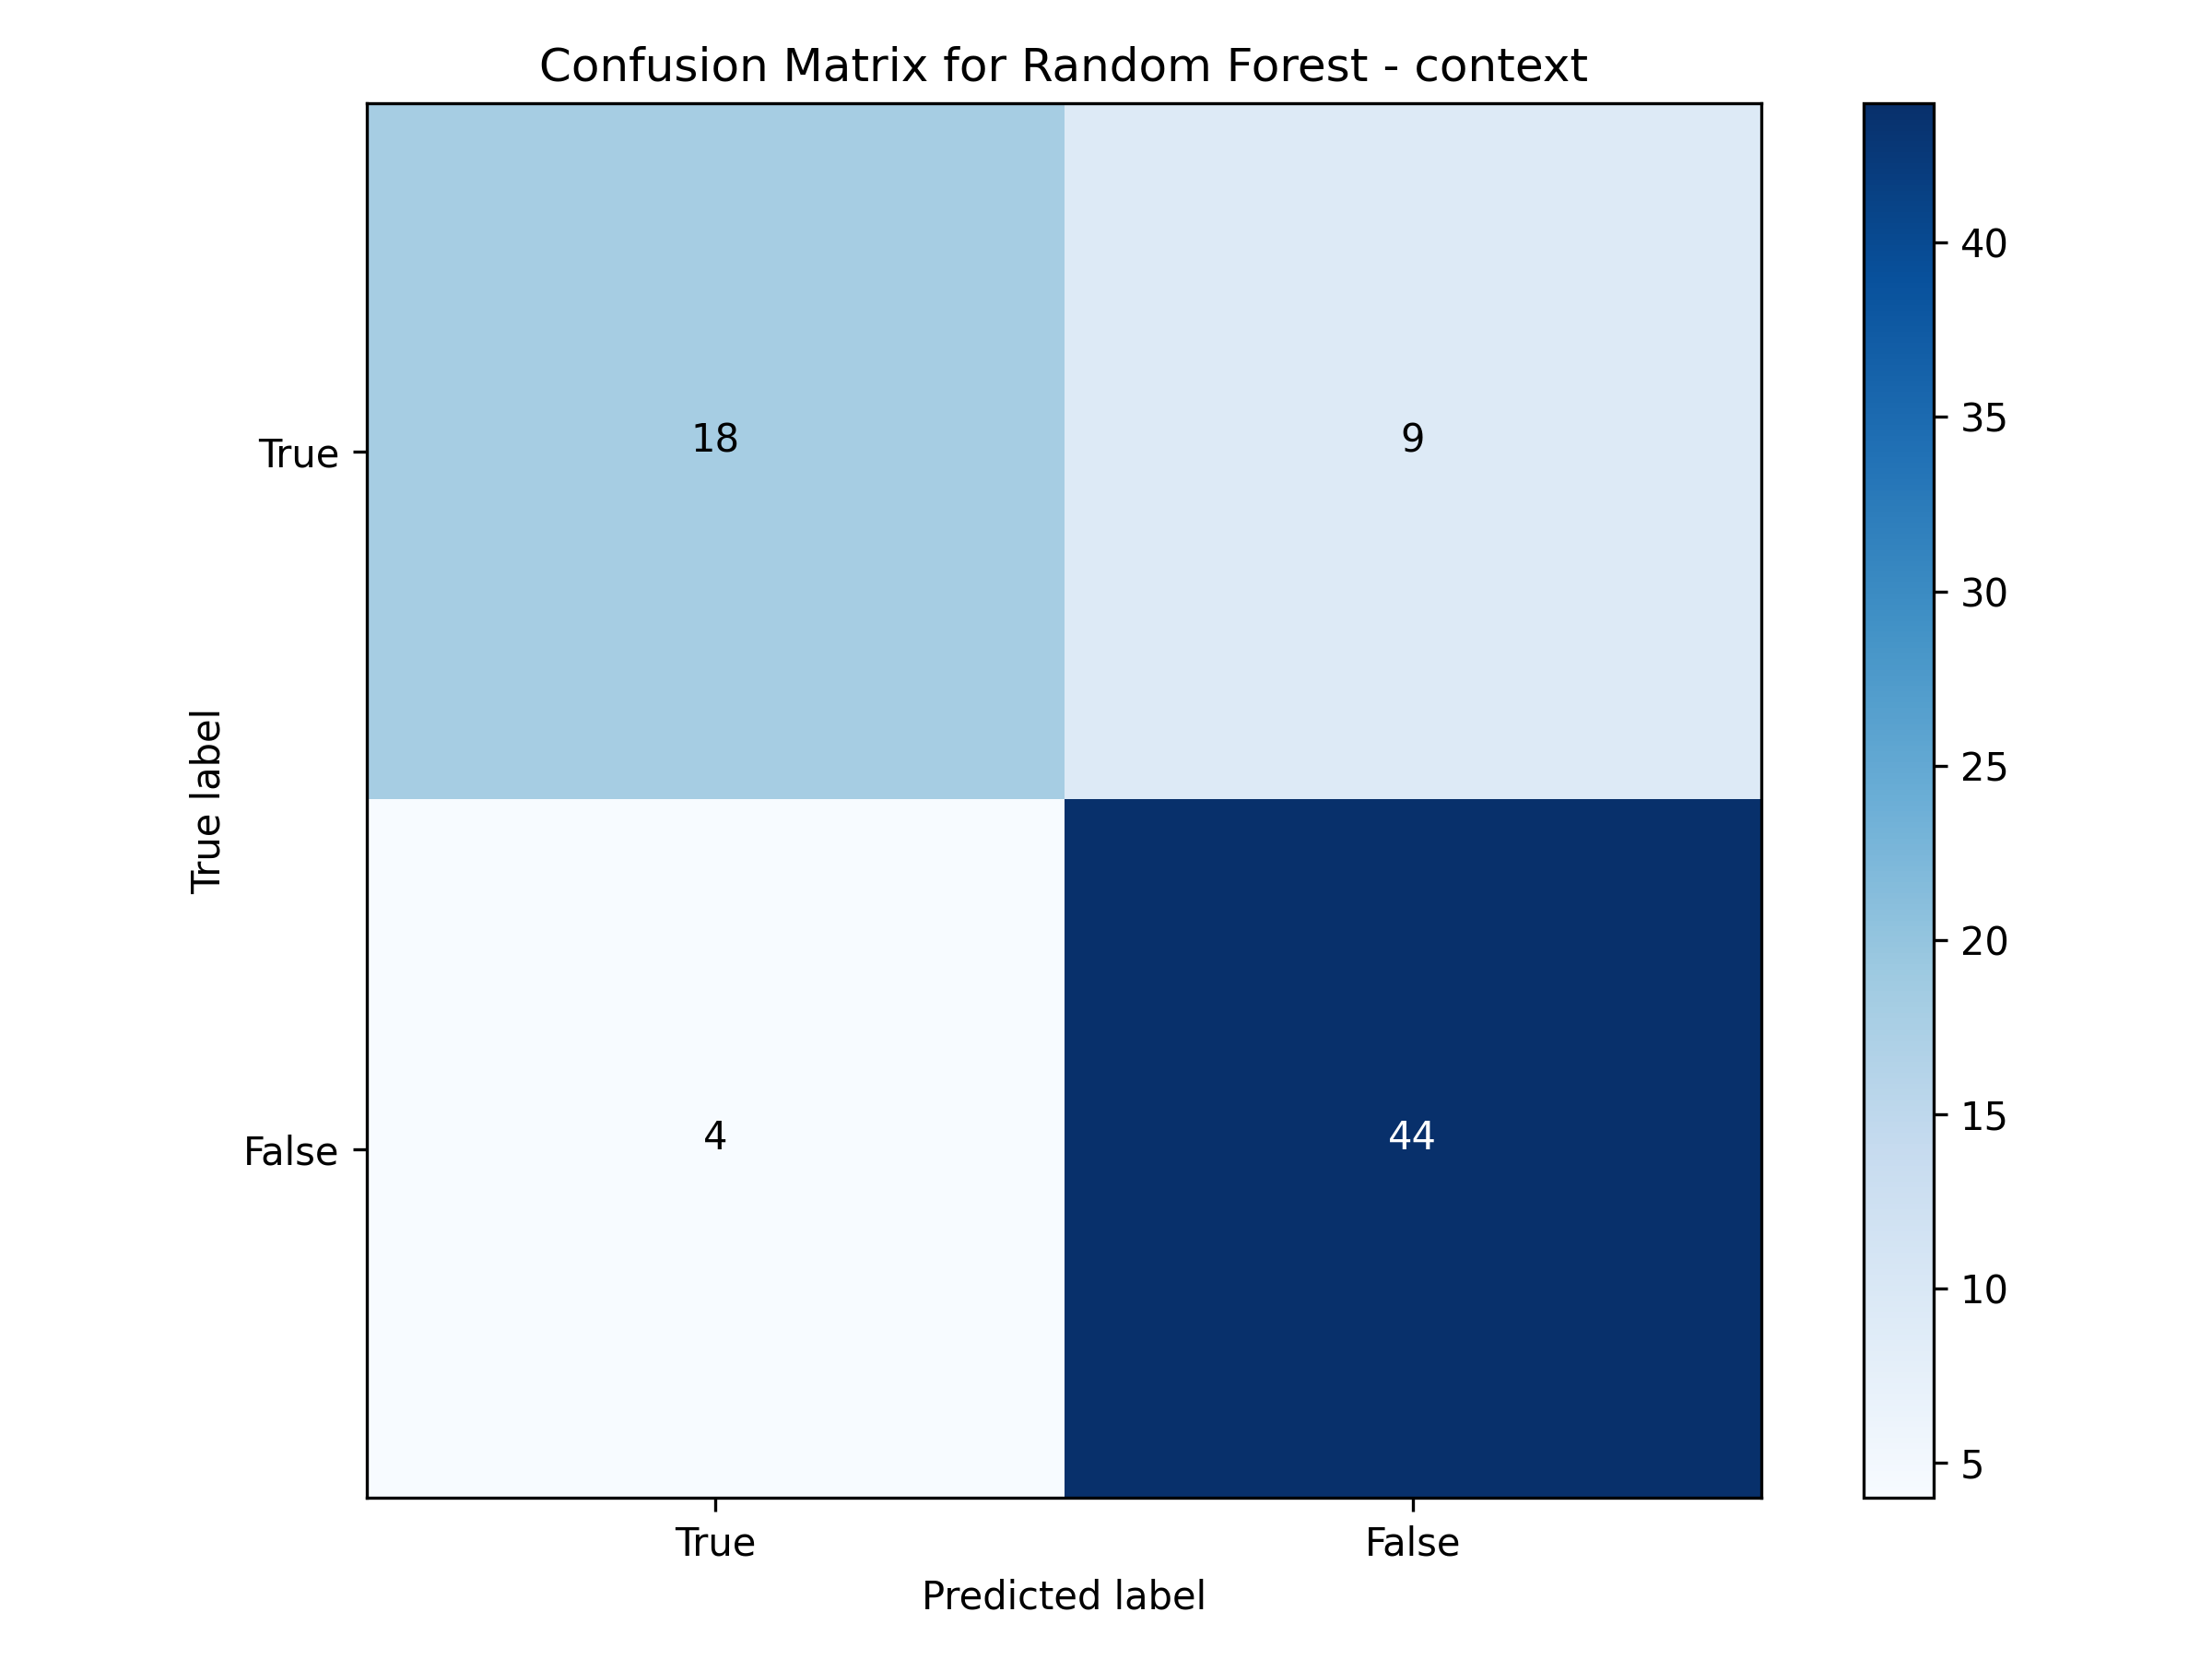
\includegraphics[width=\textwidth]{images/confusion_3.json-Random Forest_context_confusion_matrix}
        \label{fig:confusion_3_2}
    \end{minipage}
    \hspace{1em}
    \begin{minipage}[b]{0.3\textwidth}
        \centering
        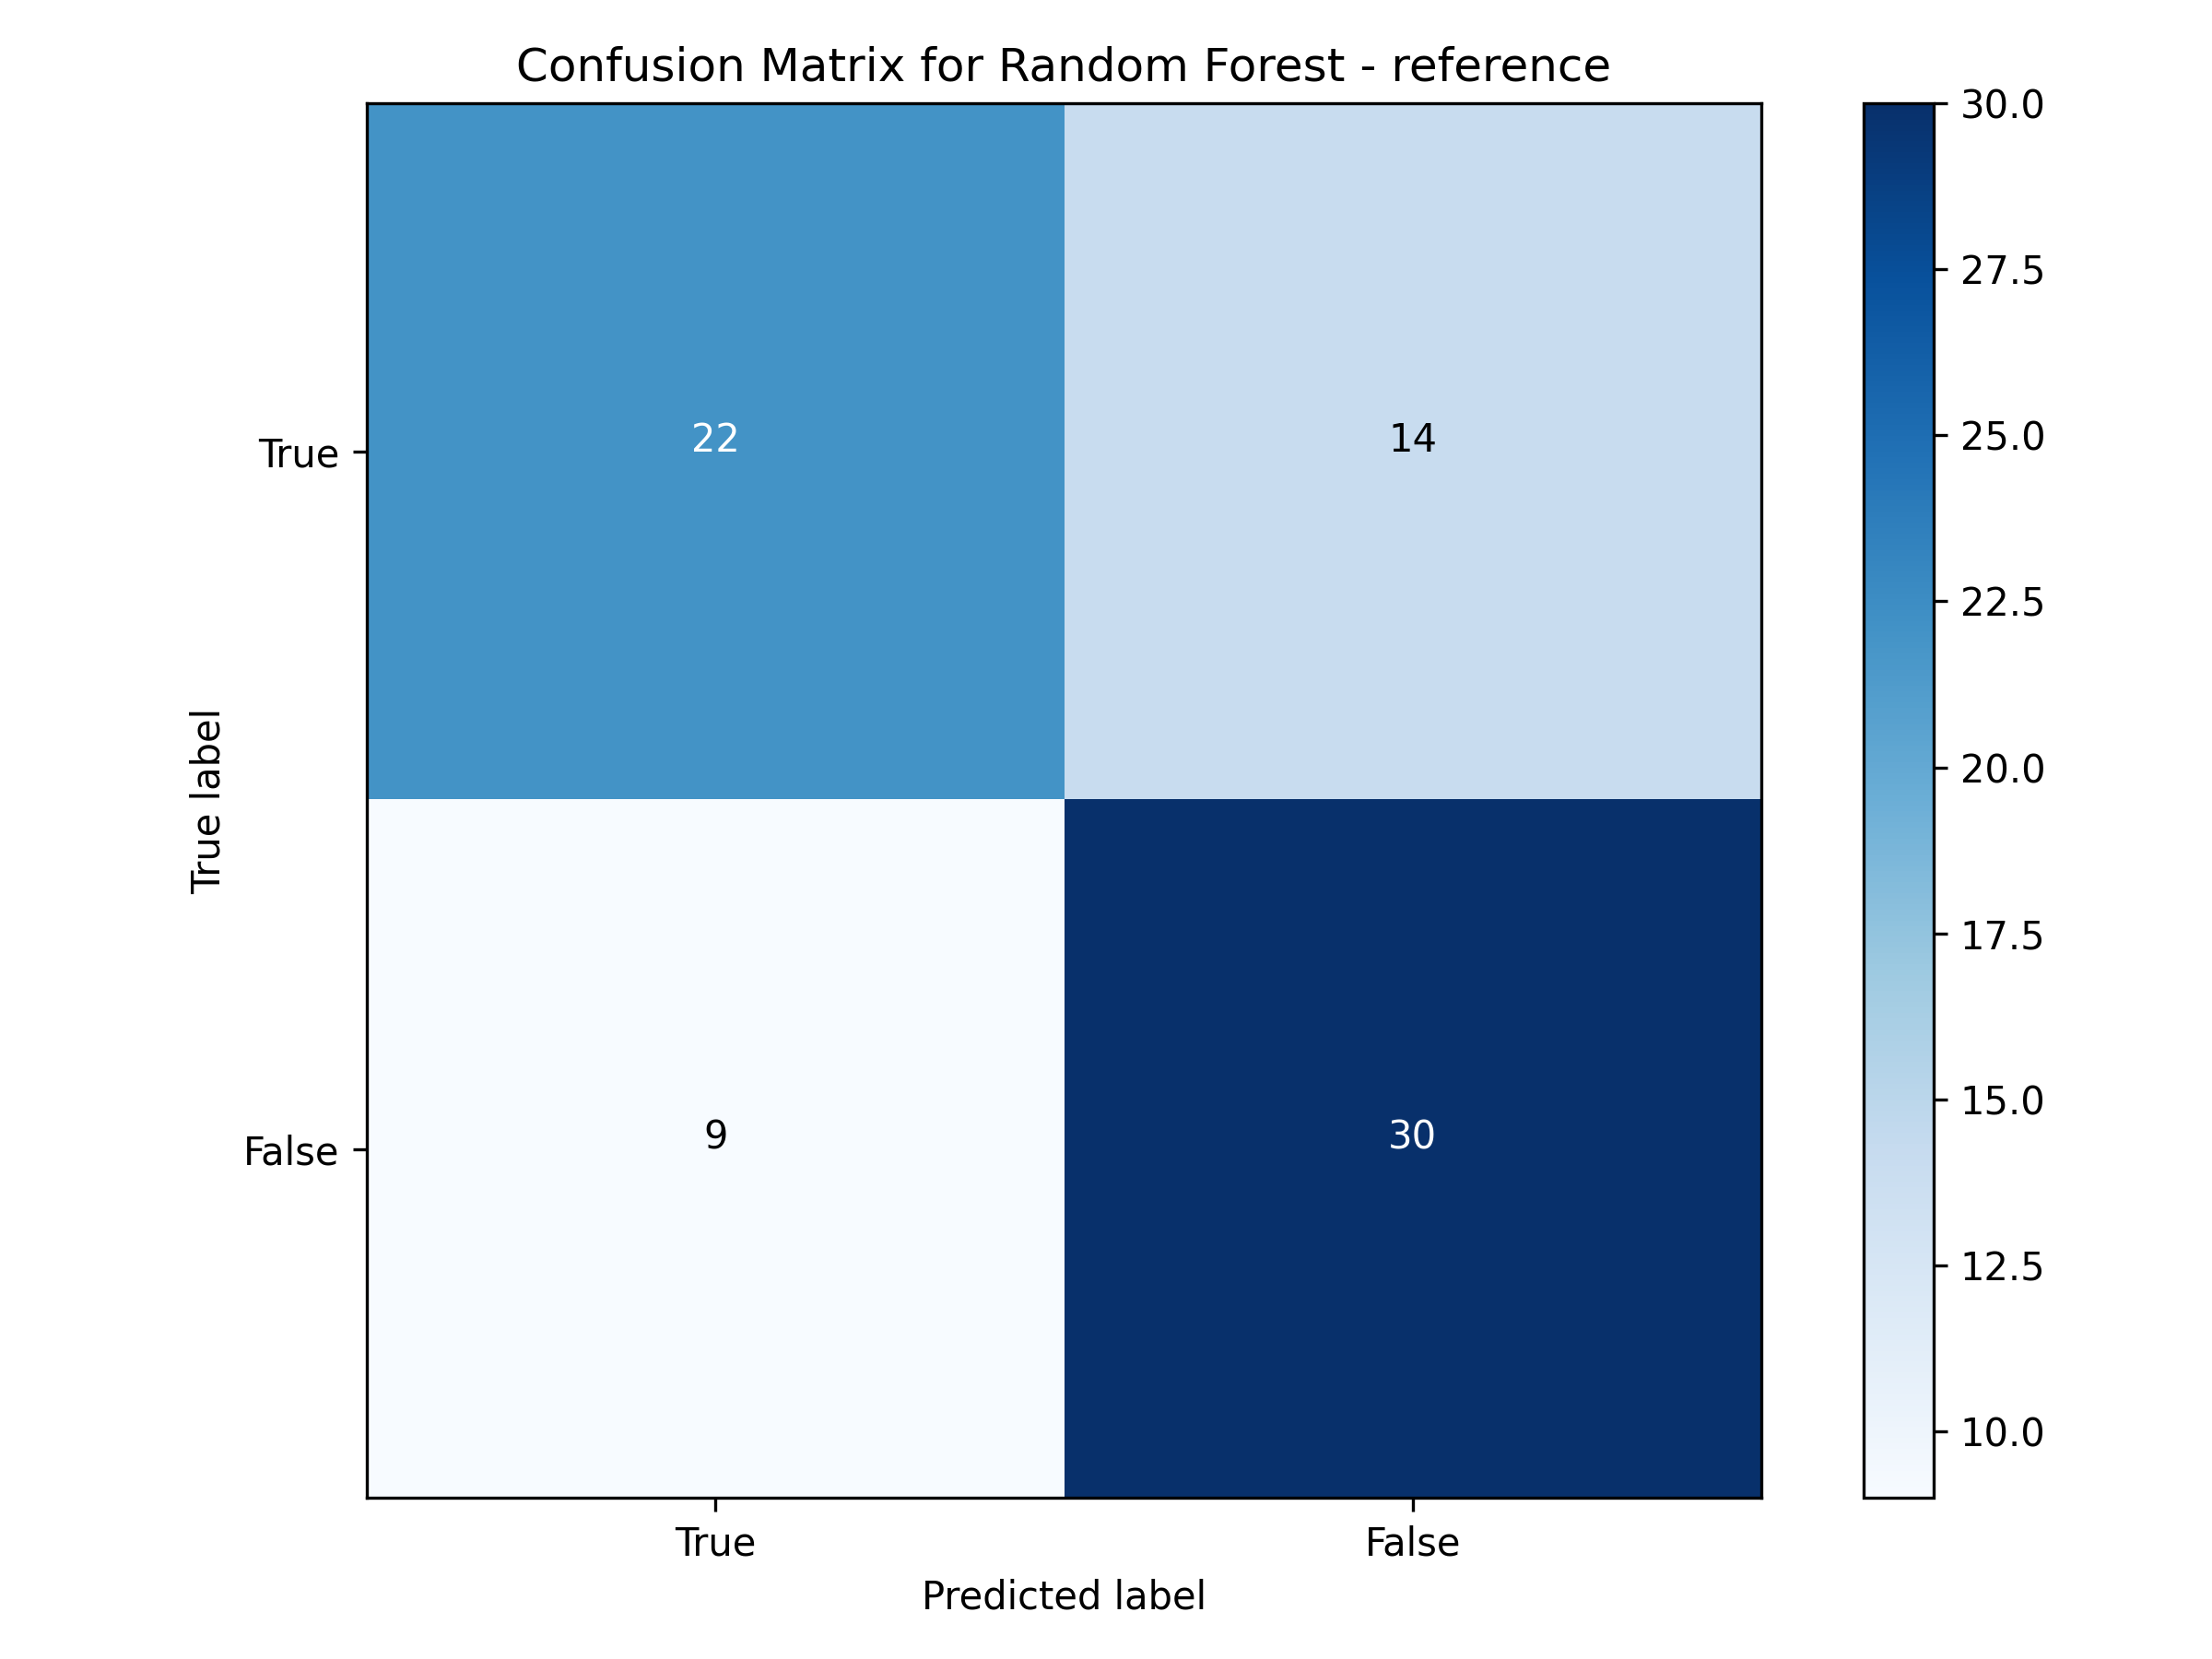
\includegraphics[width=\textwidth]{images/confusion_3.json-Random Forest_reference_confusion_matrix}
        \label{fig:confusion_3_3}
    \end{minipage}
    \caption{Matrice de confusion du modèle Random Forest pour la classification des tweets claim vs ref vs contexte.}
    \label{fig:confusion_3}
\end{figure}

Plusieurs tweets ont été mal classés selon la matrice de confusion car ils appartiennent en réalité à plusieurs classes à la fois, ce que notre système de classification a du mal à détecter simultanément.
L’accuracy, étant une métrique très stricte, pénalise fortement ce type d’ambiguïté.
Par exemple, un tweet à la fois claim et reference ne sera considéré comme bien classé que s’il est entièrement attribué à la bonne classe unique.
Nous présentons dans notre notebook une liste des tweets mal classés avec leur nombre pour illustrer cet impact.
